% !TEX root =../tfmETSI.tex
\chapter{Results and Discussion}\label{results}

% =====================================================================
%  Pass D (2026-06-07) -- second review pass folding in the user's
%  comments on Pass C+ (sections 1-15 of the consolidated fix list,
%  numbered Q1-Q7 for the open questions resolved before this rewrite).
%
%  Structure: 8 sections (Limitations moved to chapter 5; Summary table
%  folded into Discussion as 4.8.5).
%   1. Experimental Overview
%   2. Baseline
%   3. Stain normalization        (moved here -- input-side axis)
%   4. PLIP zero-shot reference
%   5. Foundational model vs plain classifier
%   6. Text encoder pretraining
%   7. Image encoder pretraining (HEADLINE)
%   8. Discussion
%
%  Per-section template (default; may collapse where uninformative):
%     Configuration -> Training source results -> Generalization to
%     external datasets -> What we learned
% =====================================================================

\providecommand{\stale}[1]{{\color{orange}#1\textsuperscript{\dag}}}
\providecommand{\todo}[1]{\textcolor{orange}{\textit{[TODO: #1]}}}
\providecommand{\pending}[1]{\textcolor{blue}{\textit{[pending: #1]}}}

% ============================================================
\section{Experimental Overview}
\label{sec:results-overview}

\subsection{Research questions}
\label{sec:results-rqs}

The chapter is built around six research questions, each targeting a single design axis of a CLIP-style histopathology pipeline: the baseline reference, the CLIP-versus-non-CLIP choice, the input-side preprocessing, the text encoder, the image encoder, and cross-dataset generalisation. Five of them (RQ1--RQ5) are answered by a dedicated experiment section in this chapter; RQ6 is cross-cutting and is addressed by the external evaluations run alongside every other experiment. The experiment matrix in Table~\ref{tab:experiment-matrix} below maps each RQ to the controlled comparison that addresses it.

\begin{itemize}
    \item \textbf{RQ1} --- What baseline classification and generalisation behaviour does a frozen general-purpose CLIP pipeline achieve on LC25000, and what failure modes appear?
    \item \textbf{RQ2} --- Does the CLIP paradigm validate its \emph{foundational-model} premise --- learning one task and generalising to tasks it was not specifically trained for --- relative to a non-CLIP classifier on the same image encoder?
    \item \textbf{RQ3} --- Does stain normalisation, an input-side preprocessing that targets a known shortcut in histopathology, help when evaluating on datasets the model was never trained on?
    \item \textbf{RQ4} --- Does using a text encoder pretrained on biomedical text (BioBERT, PubMedBERT), instead of generic BERT, improve performance under short class-name prompts?
    \item \textbf{RQ5} --- Does the image encoder's \emph{pretraining choice} matter? We test two alternatives to the ImageNet-supervised ResNet50 baseline: (a) a Visual Transformer pretrained on histopathology image--text pairs (PLIP), and (b) a Visual Transformer pretrained self-supervised on general natural images (DINOv2), which serves as a control to separate the contribution of ``ViT architecture and self-supervision'' from ``histopathology pretraining specifically''.
    \item \textbf{RQ6} --- How well does each variant generalise to data the model has never seen? We evaluate every variant against three external datasets across two organs that span shift severity: close-shift colon, different-hospital colon, and different-source lung.
\end{itemize}

\begin{table}[ht]
\centering
\small
\newcolumntype{L}[1]{>{\raggedright\arraybackslash}p{#1}}
\footnotesize
\begin{tabular}{|L{2.0cm}|L{2.4cm}|L{2.2cm}|L{1.5cm}|L{1.9cm}|L{1.9cm}|}
\hline
\textbf{Experiment} & \textbf{Image encoder} & \textbf{Text encoder} & \textbf{Loss} & \textbf{Preprocessing} & \textbf{Axis tested} \\ \hline
Baseline (\S\ref{sec:results-baseline}) & ResNet50 (ImageNet) & BERT base & InfoNCE & RGB / 255 & reference \\ \hline
Stain normalization (\S\ref{sec:results-stain}) & ResNet50 (ImageNet) & BERT base & InfoNCE & Macenko / Reinhard / Vahadane & input-side \\ \hline
PLIP zero-shot (\S\ref{sec:results-plip-zeroshot}) & ViT-B/32 (PLIP / OpenPath) & PLIP text encoder & none (zero-shot) & CLIP mean/std & reference: no LC25000 supervision \\ \hline
Foundational vs plain (\S\ref{sec:results-foundational-vs-plain}) & ResNet50 (ImageNet) & --- (no text) & cross-entropy & RGB / 255 & architecture: CLIP paradigm vs plain classifier \\ \hline
Text encoder (\S\ref{sec:results-text-encoder}) & ResNet50 (ImageNet) & BioBERT / PubMedBERT & InfoNCE & RGB / 255 & text encoder pretraining \\ \hline
Image encoder (\S\ref{sec:results-image-encoder}) & ViT-B/32 (PLIP); ViT-B/14 (DINOv2) & BERT base & InfoNCE & varies & image encoder pretraining \\ \hline
\end{tabular}
\caption{Experiment matrix. Each experiment isolates exactly one axis of variation relative to the baseline. Sections \S\ref{sec:results-baseline}--\S\ref{sec:results-image-encoder} follow this order, ending with image-encoder pretraining (the chapter's headline finding).}
\label{tab:experiment-matrix}
\end{table}

\subsection{Training source and external datasets}
\label{sec:results-ood-framework}

Every variant in this chapter is trained on a single source dataset and evaluated on three external datasets it has never seen during training. The training source is LC25000~\cite{borkowski2019lc25000}, already introduced in §\ref{sec:results-baseline-config}: every trained variant is fit on it, and the in-distribution test split yields the macro-F1 we refer to as \emph{training-source results} throughout the chapter. The three external datasets --- the source of every \emph{generalisation} number in the chapter --- are listed in order of shift severity:

\begin{itemize}
    \item \textbf{NCT-CRC-HE-7K}~\cite{kather2019nct}, close-shift colon: $1\,974$ scored patches over the \texttt{NORM} and \texttt{TUM} classes, mapping to \emph{benign colon tissue} and \emph{colon adenocarcinoma} in LC25000.
    \item \textbf{Chaoyang}~\cite{zhu2021chaoyang}, different-hospital colon: $4\,060$ scored patches (\texttt{normal} and \texttt{adenocarcinoma}; the \texttt{serrated} and \texttt{adenoma} classes have no clean LC25000 analogue and are excluded from scoring), mapping to the same two LC25000 colon classes as NCT.
    \item \textbf{LungHist700}~\cite{tabatabaei2024lunghist}, different-source lung: $359$ images at $20\times$ magnification (the $40\times$ subset is excluded), mapping to LC25000's \emph{benign lung tissue}, \emph{lung adenocarcinoma}, and \emph{lung squamous cell carcinoma}.
\end{itemize}

Full dataset provenance, acquisition details, and per-dataset preprocessing live in Methodology (§\ref{sec:meth-external-datasets}); the bullets above keep only what is needed to interpret the external-evaluation tables in the rest of the chapter.

Three protocol choices apply to every external evaluation that follows. First, \textbf{restricted argmax}: each variant exposes all $5$ LC25000 class prompts at inference, but the argmax is restricted to the LC25000 classes that map to the external dataset's organ ($2$ colon classes for NCT and Chaoyang, $3$ lung classes for LungHist700). Predictions into a non-target LC25000 class count as wrong but are reported separately when informative for confusion analysis. Second, \textbf{pure inference}: every variant reuses its LC25000-trained checkpoint without further adaptation; no fine-tuning is performed on the external datasets. Third, \textbf{per-dataset reporting}: results are presented per dataset rather than averaged. The motivation for that last choice is methodological --- aggregating across datasets would average a colon-side partial transfer ($\sim 0.79$--$0.87$ F1) with a lung-side categorical failure ($0.305$ F1 in the baseline), producing a single mean-OOD number that hides the cross-organ regime change that ends up driving the chapter's headline result in §\ref{sec:results-image-encoder}.

\subsection{Metrics and visualizations}
\label{sec:results-metrics}

Each variant in this chapter is reported with the same set of metrics and visualisations. The choices and what each is meant to surface:
\begin{itemize}
    \item \textbf{Macro-F1} is the headline metric. It averages the per-class F1 scores equally, which is the right behaviour for the per-class precision--recall trade-offs that drive the chapter's substantive comparisons. Formal definitions are in Methodology (§\ref{sec:meth-eval}).
    \item \textbf{Accuracy, balanced accuracy, weighted F1, and per-class precision/recall/F1} are reported alongside macro-F1 for completeness, but the chapter's interpretive weight is on macro-F1 and the per-class numbers.
    \item \textbf{Confusion matrices} (raw counts and row-normalised by true class) are reported per variant and per dataset --- the most direct view of how a model distributes its errors across the available classes.
    \item \textbf{Training-source UMAP} projects LC25000 image embeddings and class-prompt embeddings into the same 2-D fit (cosine metric), letting the reader see cluster separation and the alignment between image clusters and prompt anchors.
    \item \textbf{Cross-distribution UMAP grid} (per external dataset, per variant) overlays LC25000 dots and external-dataset triangles in a single 2-D fit, asking whether the external dataset co-locates with the matching LC25000 class cluster or sits in its own region of feature space.
\end{itemize}


% ============================================================
\section{Baseline: frozen ResNet50 and frozen BERT}
\label{sec:results-baseline}

\subsection{Configuration}
\label{sec:results-baseline-config}

The baseline pipeline pairs a frozen ResNet50 image encoder, taken from the standard ImageNet-supervised checkpoint, with a frozen BERT-base-uncased text encoder; only a pair of small projection heads --- a single $256$-wide \texttt{Dense} layer with no bias, followed by \texttt{LayerNorm} --- and a scalar temperature $\tau$ are trained on top. This is deliberately the most general-purpose CLIP one can assemble. ResNet50 is the canonical CNN baseline of the past decade and BERT-base is the canonical text encoder; neither has been exposed to histology during pretraining, and neither has been tuned for the task. The reason to start here is mechanical: every subsequent variant in this chapter changes exactly one piece of this configuration, and the resulting delta is only interpretable if the reference is something recognisable rather than something already adapted to the data.

Everything else is held constant across the variants that follow. The training data is the LC25000 dataset, with a $80/10/10$ train--validation--test split at random seed $42$; a single fixed composed prompt, \texttt{``A histopathology image of \{class\_name\}.''}, is used at both training and inference; the loss is symmetric InfoNCE; the optimiser is AdamW with learning rate $1 \times 10^{-3}$ and weight decay $1 \times 10^{-4}$; and training runs for at most $30$ epochs, with EarlyStopping (patience $5$, restore best weights) terminating it earlier on every run. The remaining design choices --- batch size, image and sequence dimensions, initial temperature, gradient clipping, learning-rate schedule, numerical precision, weight initialisation --- are not referenced again in this chapter and are gathered in the baseline hyperparameter table in Methodology (Table~\ref{tab:baseline-hyperparameters}).

\subsection{Training behaviour and in-distribution results}
\label{sec:results-baseline-training}

On the LC25000 test split, the baseline reaches a macro-F1 of $0.996$. The model has only two trainable projection heads and a scalar temperature $\tau$ on top of frozen encoders --- around $720{,}000$ parameters in total --- so a saturated in-distribution score would invite a memorisation reading without a check on the training dynamics. Figure~\ref{fig:baseline-loss} provides that check: the training and validation InfoNCE losses (equation~\eqref{eq:infonce-sym}) descend together over the $30$-epoch budget and stay close at convergence. The learnable temperature $\tau$ (equation~\eqref{eq:scaled-cosine}), initialised at the CLIP-paper value of $0.07$, \emph{rises} during training, peaks at $\approx 0.090$ around epoch $10$, and settles near $0.087$. This is the opposite direction from the CLIP paper's $\tau \to 0.01$ behaviour on uniquely-paired image--text data, and is consistent with our shared-prompt setup: when multiple images per batch share the same class prompt (the false-negative caveat in §\ref{sec:meth-clip}), softening $\tau$ reduces the penalty those false negatives impose on otherwise-correct alignments.

\begin{figure}[H]
    \centering
    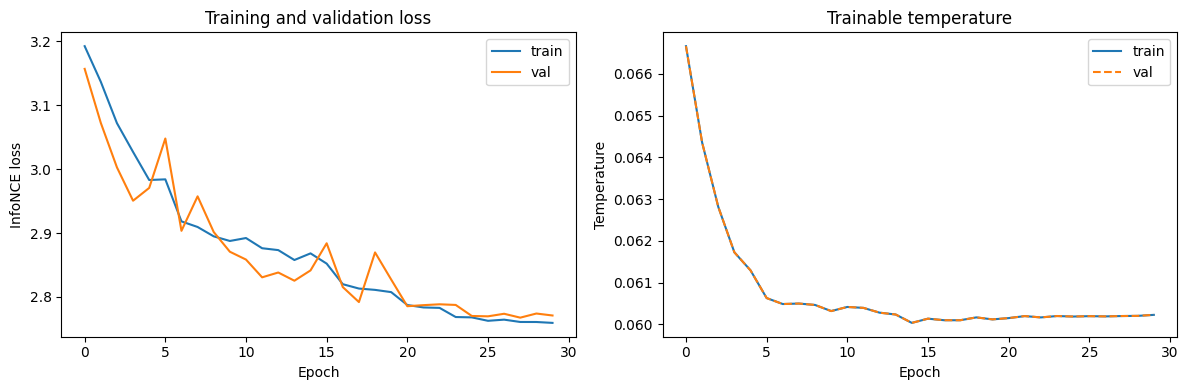
\includegraphics[width=0.9\textwidth]{../results/plots/baseline_loss.png}
    \caption{Baseline training (blue) and validation (orange) InfoNCE loss across epochs (left), and the learnable temperature $\tau$ on the same horizontal axis (right).}
    \label{fig:baseline-loss}
\end{figure}

The embedding space the model converges to is shown in Figure~\ref{fig:baseline-umap}. Each LC25000 class forms a distinct cluster of image embeddings and the five class-prompt anchors (encoded through frozen BERT and projected to the same $256$-d space) sit at the centre of their corresponding clusters --- the expected post-InfoNCE alignment between text and image, with the trained projection heads doing the work that the frozen text encoder alone could not. The lung-adenocarcinoma cluster sits closest to lung squamous cell carcinoma in the 2D projection, foreshadowing the off-diagonal confusion-matrix mass discussed below.

\begin{figure}[H]
    \centering
    \begin{minipage}[t]{0.48\textwidth}
        \centering
        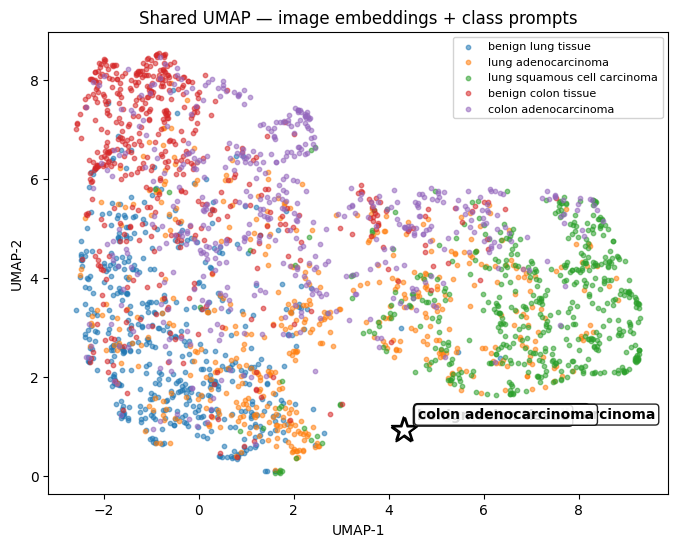
\includegraphics[width=\textwidth]{../results/plots/baseline_umap.png}
        \par\vspace{2pt}\footnotesize (a) Vanilla scatter.
    \end{minipage}\hfill
    \begin{minipage}[t]{0.48\textwidth}
        \centering
        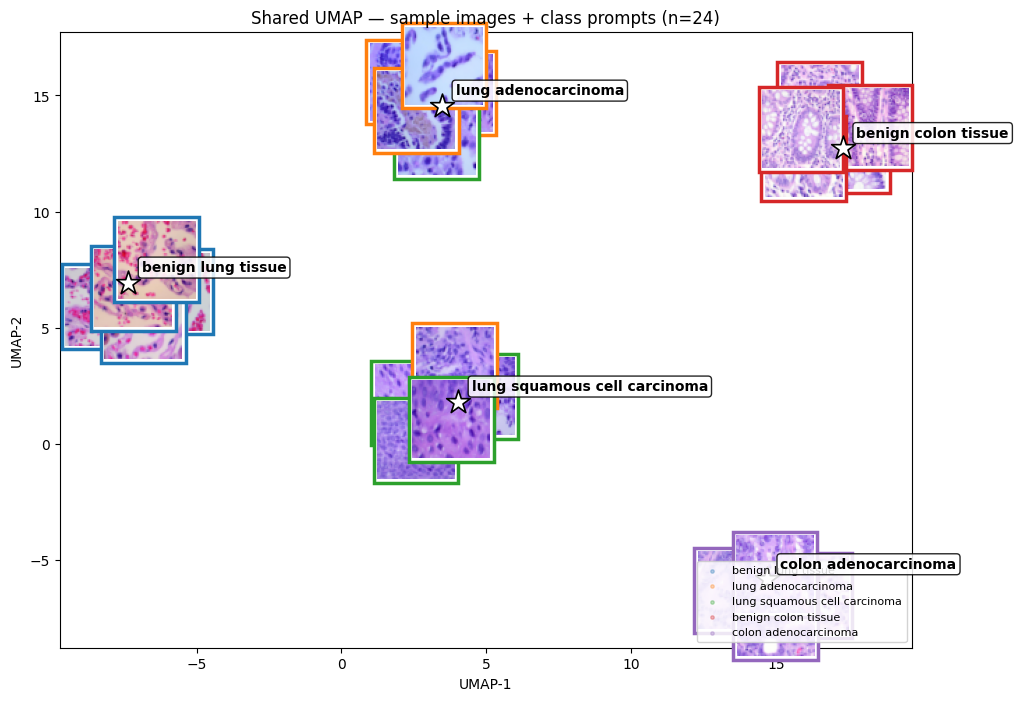
\includegraphics[width=\textwidth]{../results/plots/baseline_umap_thumbnails.png}
        \par\vspace{2pt}\footnotesize (b) Sample-image thumbnails.
    \end{minipage}
    \caption{UMAP of the baseline embedding space on the LC25000 test split. Two views of the same fit: (a) per-class scatter with the five class-prompt anchors marked, (b) the same fit overlaid with sample-image thumbnails.}
    \label{fig:baseline-umap}
\end{figure}

The confusion matrix (Figure~\ref{fig:baseline-cm}) confirms that the saturated $0.996$ is genuinely close to ceiling: the benign tissues and lung squamous cell carcinoma separate cleanly, with the off-diagonal mass concentrated on lung adenocarcinoma --- the hardest discrimination in the LC25000 schema. In-distribution, thus, does not discriminate the baseline from any of the trained variants studied in subsequent sections (all of them saturate at $\sim 0.99$); the meaningful comparison is the external evaluation that follows in §\ref{sec:results-baseline-ood}.

\begin{figure}[H]
    \centering
    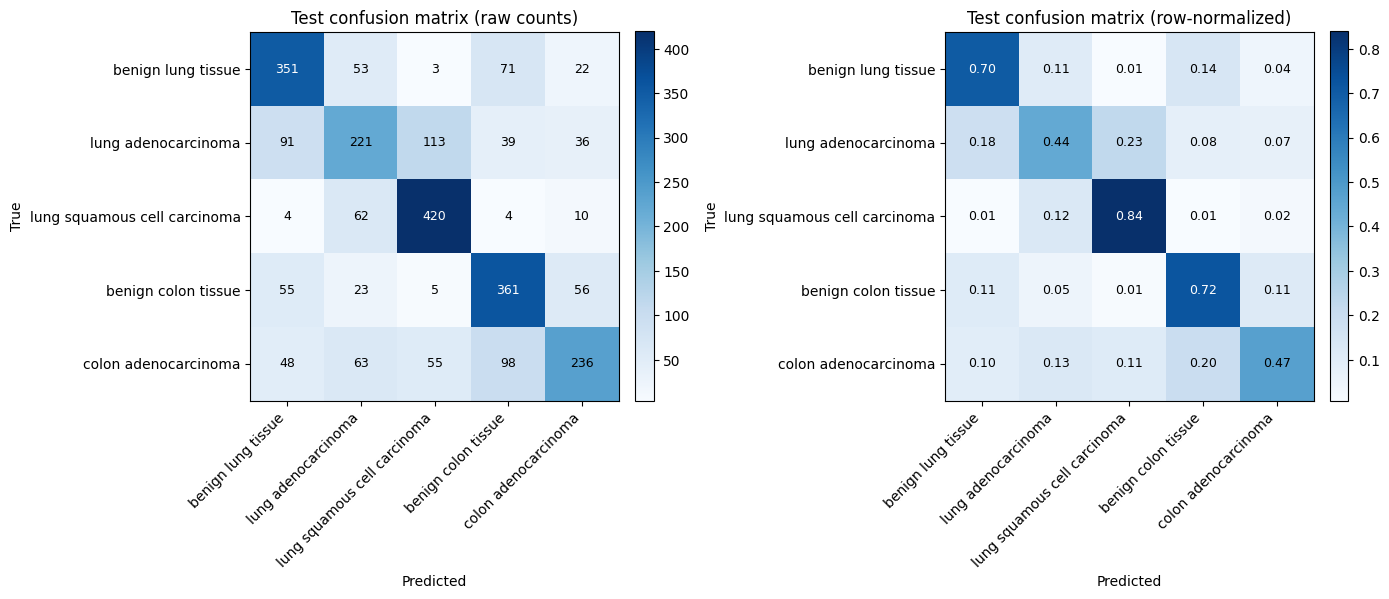
\includegraphics[width=0.95\textwidth]{../results/confusion_matrices/baseline_confusion_matrices.png}
    \caption{Baseline confusion matrix on the LC25000 test split. Left: raw counts. Right: row-normalised by true class.}
    \label{fig:baseline-cm}
\end{figure}

\FloatBarrier
\subsection{Generalization to external datasets}
\label{sec:results-baseline-ood}

The baseline's macro-F1 on each external dataset, restricted-argmax over the target-organ LC25000 classes, is reported in Table~\ref{tab:baseline-ood}. The result splits in two. On the two colon datasets the baseline transfers partially --- $0.866$ on NCT-CRC-HE-7K, the dataset stylistically closest to LC25000's colon distribution, and $0.786$ on Chaoyang, where a different hospital, scanner, and staining protocol drag the score down by $\sim 0.08$ F1 even though the organ is unchanged. On lung the picture is qualitatively different: \textbf{$\mathbf{0.305}$ macro-F1 on LungHist700's 3-class problem, where chance is $\mathbf{0.33}$}. The colon-versus-lung gap dwarfs every within-organ shift in the table --- the central observation the rest of the chapter sets out to explain.

\begin{table}[H]
    \centering
    \small
    \begin{tabular}{|l|c|c|c|c|}
    \hline
    \textbf{External dataset (organ)} & \textbf{Macro-F1} & \textbf{Accuracy} & \textbf{Bal.\ acc.} & \textbf{Weighted F1} \\ \hline
    NCT-CRC-HE-7K (colon)            & \textbf{0.866} & 0.870 & 0.866 & 0.871 \\ \hline
    Chaoyang (colon)                 & \textbf{0.786} & 0.796 & 0.782 & 0.791 \\ \hline
    LungHist700 (lung, 20$\times$)   & \textbf{0.305} & 0.390 & 0.383 & 0.301 \\ \hline
    \end{tabular}
    \caption{Baseline generalization to the three external datasets, restricted-argmax over the target-organ LC25000 classes.}
    \label{tab:baseline-ood}
\end{table}

The lung results are not a noisy degradation of the colon transfer; they are a different failure mode. Per-class recall on LungHist700 breaks down as $0.89$ for lung squamous cell carcinoma, $0.07$ for lung adenocarcinoma, and $0.19$ for benign lung tissue. Back-calculated from the precision figures, \textbf{the model assigns ``squamous'' to roughly $\mathbf{84}$\% of LungHist700 inputs regardless of true class} --- and given that squamous accounts for only $36$\% of the ground truth, the near-chance macro-F1 is the direct consequence of that bias. Figure~\ref{fig:baseline-lung-umap} shows the matching feature-space signature: all $359$ LungHist700 samples collapse into a single tight cluster with no visible internal class structure. The frozen ImageNet-supervised ResNet50, never exposed to histology during pretraining, extracts no usable per-class variance from LungHist700 tissue, and the trained projection head has nothing to align with the three lung class prompts.

\begin{figure}[H]
    \centering
    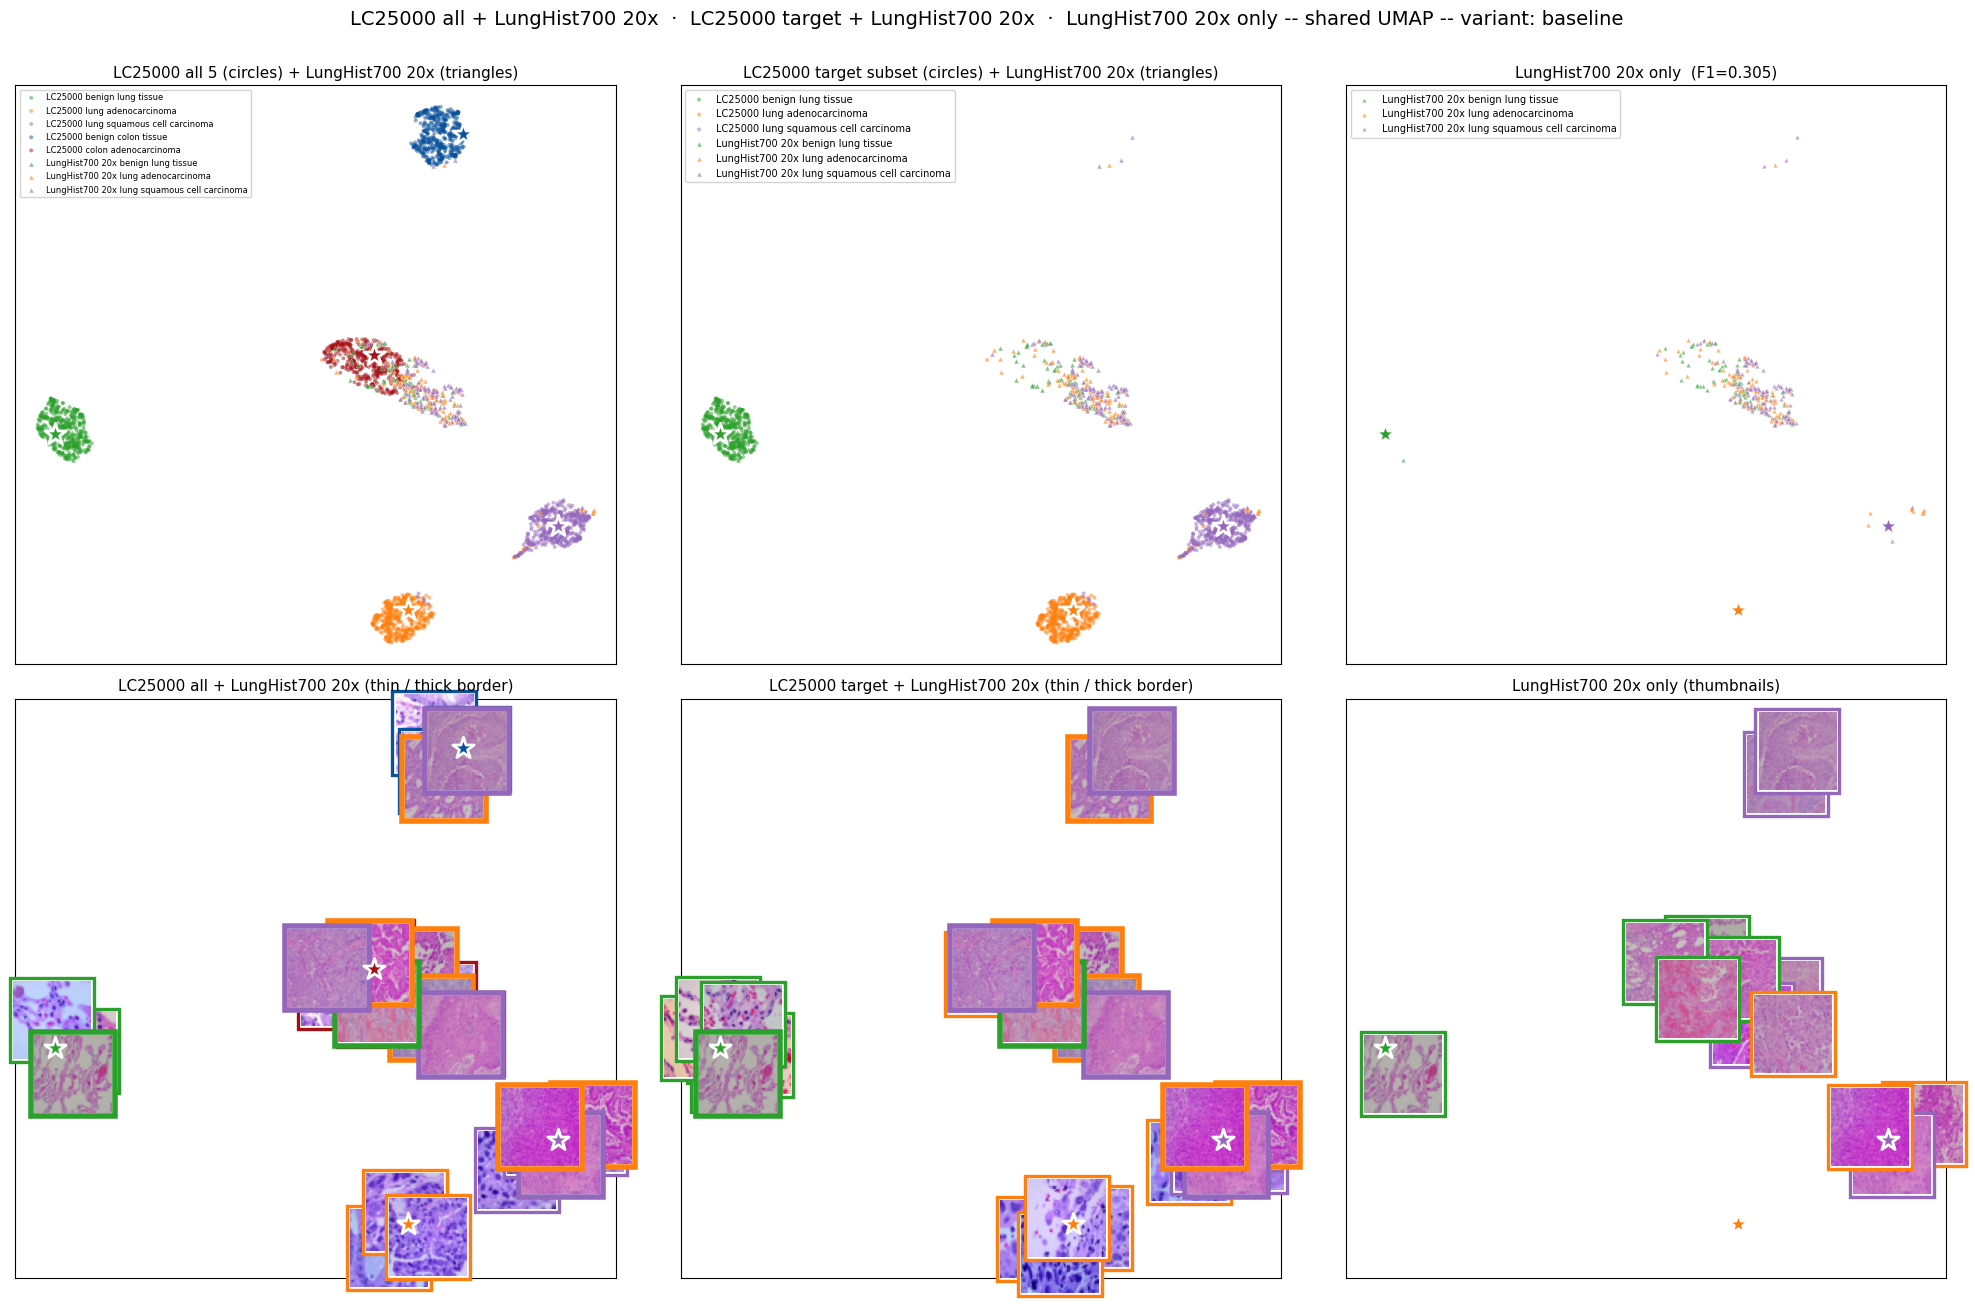
\includegraphics[width=0.95\textwidth]{../results/plots/exp_07_ood_eval/baseline_lunghist700_20x_ood_umap_grid.png}
    \caption{Baseline cross-distribution UMAP on LungHist700. LC25000 image embeddings (dots) and LungHist700 image embeddings (triangles) projected into the same 2-D fit.}
    \label{fig:baseline-lung-umap}
\end{figure}

The Chaoyang dataset sits between these two regimes (Figure~\ref{fig:baseline-chaoyang-umap}). The two colon classes are partially separated in the projected space, and the Chaoyang triangles cluster in a region adjacent to --- but not co-located with --- the matching LC25000 colon clusters: enough signal for partial transfer, with a measurable cost from the cross-hospital distribution gap. Together with NCT and LungHist700, this exposes two distinct generalisation regimes for the experiments that follow. There is a colon regime, where frozen ImageNet features carry good-enough structure for partial transfer, and a lung regime, where they carry no usable structure at all. The central question the rest of this chapter is built around: is the lung-side failure about the encoder's architecture, about its supervised pretraining on natural images, or about the absence of histopathology data in pretraining? The DINOv2 control (general-domain self-supervised pretraining, no histology) and the PLIP backbone (ViT pretrained on histopathology image--text pairs) jointly decompose that question, and the headline answer arrives in §\ref{sec:results-image-encoder}.

\begin{figure}[H]
    \centering
    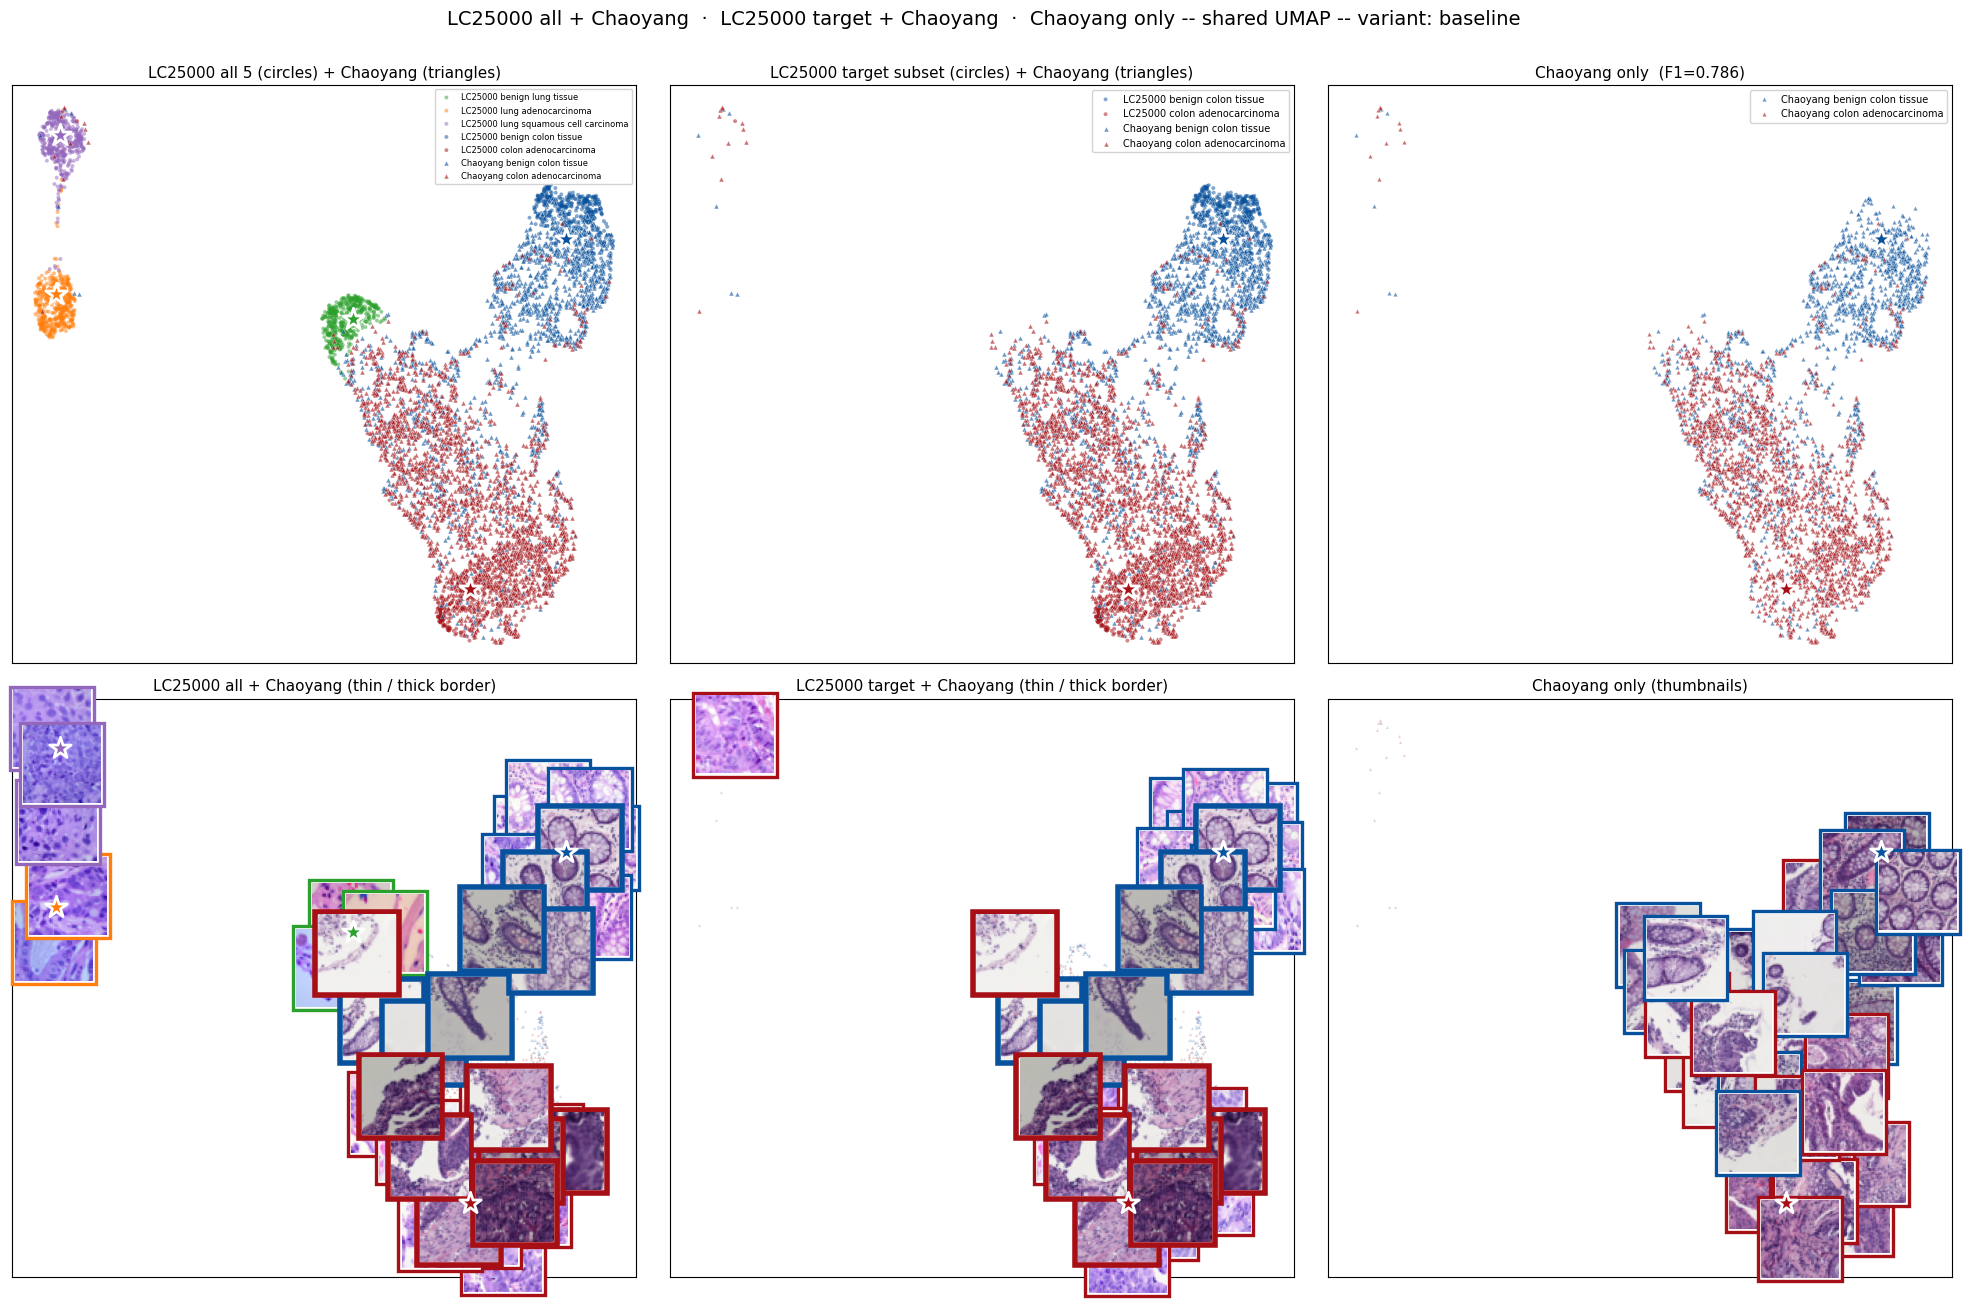
\includegraphics[width=0.95\textwidth]{../results/plots/exp_07_ood_eval/baseline_chaoyang_ood_umap_grid.png}
    \caption{Baseline cross-distribution UMAP on Chaoyang. LC25000 image embeddings (dots) and Chaoyang image embeddings (triangles) projected into the same 2-D fit.}
    \label{fig:baseline-chaoyang-umap}
\end{figure}


% ============================================================
\FloatBarrier
\section{Stain normalization}
\label{sec:results-stain}

\subsection{Configuration}

The stain-normalisation experiment keeps the baseline pipeline architecture identical to §\ref{sec:results-baseline-config} and changes only the image-input distribution. Every LC25000 training image is Macenko-normalised~\cite{macenko2009stain} against a single fixed reference patch: the first \texttt{NORM} tile from NCT-CRC-HE-7K, abbreviated ``NCT-NORM'' below.

The choice of reference matters operationally. NCT-CRC is distributed already Macenko-normalised against an unpublished Kather-team reference~\cite{kather2019nct}; by Macenko-normalising LC25000 onto an NCT-CRC tile, we land the training distribution in approximately the colour space NCT-CRC arrives in at release, which lets NCT-CRC be fed raw at evaluation and avoids the double-Macenko regime that historically zeroed out the OOD F1 in an earlier version of this experiment. Chaoyang and LungHist700, by contrast, arrive in their native un-normalised palettes, so for those two datasets the same Macenko(NCT-NORM) transform is applied at inference to bring them into the model's training-stain space. An alternative reference drawn from Chaoyang or LungHist700 --- the latter being the most stain-distinct of the three external datasets --- would have re-introduced the double-Macenko problem on NCT-CRC and required a separate retraining run for each reference tested; the NCT-NORM reference is therefore picked for methodological consistency rather than per-dataset optimisation, and reference rotation as an ablation axis is documented as a limitation in Chapter~\ref{chp:conclusion}.

Reinhard and Vahadane were also explored as alternative normalisations in an exploratory pass but did not advance to the full external-evaluation ablation. Vahadane's NMF solver fails to converge on a fraction of LC25000 patches --- visible in Figure~\ref{fig:stain-before-after}(d), where the bottom-row \texttt{colon\_aca} cell re-renders near-blank. Reinhard is a Lab-space colour-statistics transfer rather than a stain-decomposition method, included in the figure for visual comparison only.

\begin{figure}[ht]
    \centering
    \begin{minipage}[t]{0.23\textwidth}
        \centering
        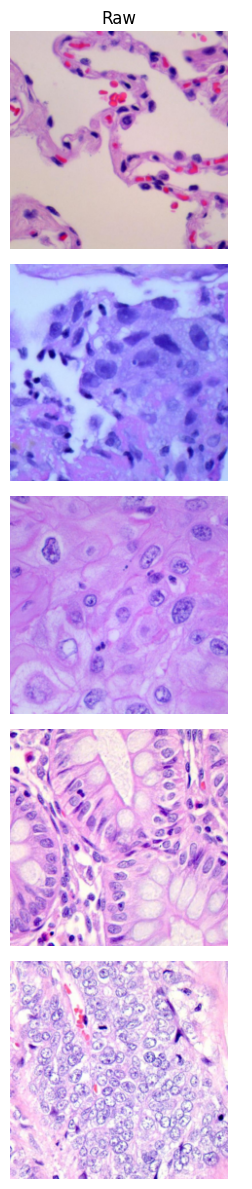
\includegraphics[width=\textwidth]{../results/plots/stain_raw_examples.png}
        \par\vspace{2pt}\footnotesize (a) Raw.
    \end{minipage}\hfill
    \begin{minipage}[t]{0.23\textwidth}
        \centering
        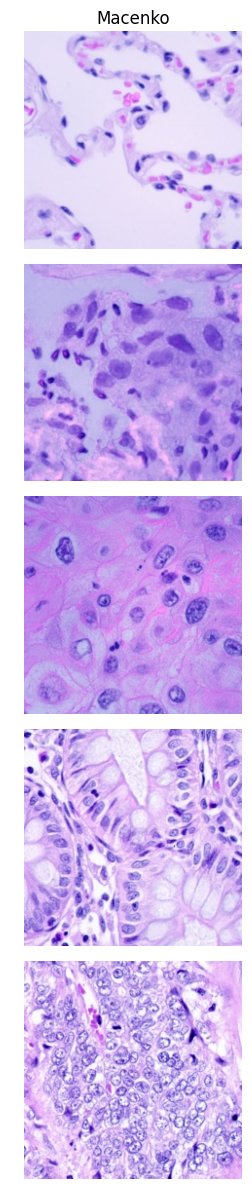
\includegraphics[width=\textwidth]{../results/plots/stain_macenko_normalized_only.png}
        \par\vspace{2pt}\footnotesize (b) Macenko.
    \end{minipage}\hfill
    \begin{minipage}[t]{0.23\textwidth}
        \centering
        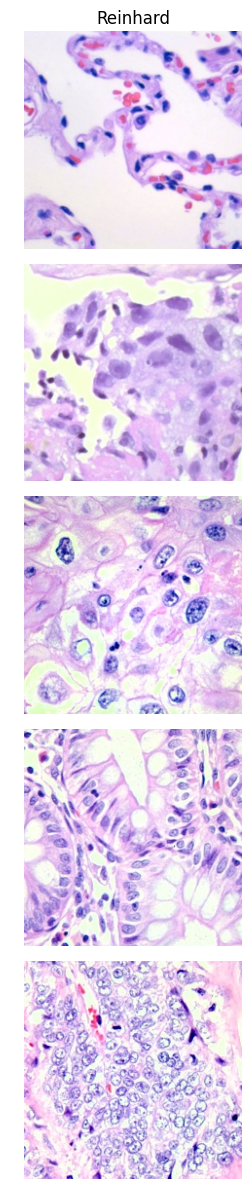
\includegraphics[width=\textwidth]{../results/plots/stain_reinhard_normalized_only.png}
        \par\vspace{2pt}\footnotesize (c) Reinhard.
    \end{minipage}\hfill
    \begin{minipage}[t]{0.23\textwidth}
        \centering
        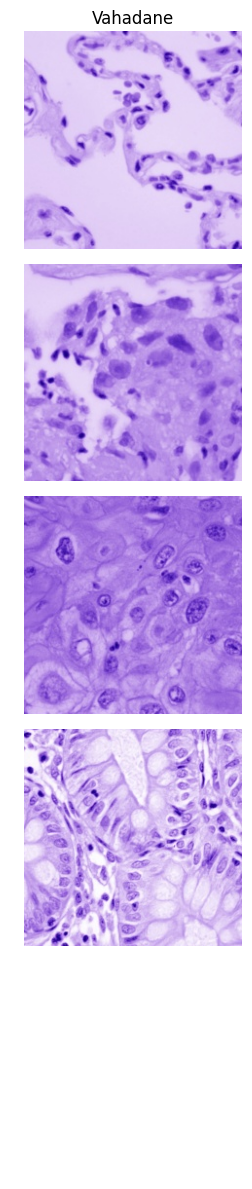
\includegraphics[width=\textwidth]{../results/plots/stain_vahadane_normalized_only.png}
        \par\vspace{2pt}\footnotesize (d) Vahadane.
    \end{minipage}
    \caption{Stain normalization, one example per class. Column (a) shows the raw inputs (identical across methods, shown once for compactness); columns (b)--(d) show the same inputs after Macenko, Reinhard, and Vahadane normalization respectively. The bottom-row colon\_aca cell in column (d) shows the Vahadane NMF solver failing to converge and re-rendering near-blank, an instability discussed in the interpretation.}
    \label{fig:stain-before-after}
\end{figure}

\subsection{Generalization to external datasets}

On LC25000 the Macenko-trained checkpoint saturates at $0.986$ macro-F1, alongside the baseline and every other trained variant in this study --- in-distribution does not discriminate this lever, so the substantive comparison is the external evaluation reported in Table~\ref{tab:stain-3way}.

\begin{table}[H]
    \centering
    \small
    \begin{tabular}{|l|c|c|c|}
    \hline
    \textbf{External dataset} & \textbf{Baseline F1} & \textbf{Macenko F1} & \textbf{Delta} \\ \hline
    NCT-CRC-HE-7K (close-shift colon)         & $0.866$ & $0.844$ & $-0.022$ \\ \hline
    Chaoyang (different-hospital colon)       & $0.786$ & $0.816$ & $+0.030$ \\ \hline
    LungHist700 (different-source lung, 20$\times$)  & $0.305$ & $0.325$ & $+0.020$ \\ \hline
    \end{tabular}
    \caption{Macenko(NCT-NORM) vs baseline on the three external evaluation datasets.}
    \label{tab:stain-3way}
\end{table}

\textbf{The lever's direction is data-dependent.} On the two datasets that arrive in their native stain palette --- Chaoyang ($+0.030$ F1) and LungHist700 ($+0.020$ F1), both receiving Macenko at inference --- normalisation moves the input closer to the model's training distribution and the frozen ImageNet ResNet50 produces better features. On NCT-CRC the picture inverts: NCT was already in approximately the target stain space at release, so training-time Macenko introduced a non-linear shift the frozen backbone could not absorb, and the eval-time pass-through cannot recover the small cost paid ($-0.022$ F1).

The magnitude is modest, even where the lever helps. The $+0.020$--$+0.030$ F1 gains on Chaoyang and LungHist700 are real but small; by comparison, swapping the image encoder to PLIP (§\ref{sec:results-image-encoder}) gains $+0.027$ on Chaoyang and \textbf{$\mathbf{+0.335}$ on LungHist700 --- an order of magnitude larger}. At the frozen-backbone scale evaluated here, stain normalisation is a useful but not dominant lever, and the protocol lesson worth carrying forward is the asymmetric application: Macenko is applied at inference only on inputs that arrive in their native stain palette, since doubling on a pre-normalised target is what historically broke the OOD F1 in this experiment.


% ============================================================
\section{PLIP zero-shot reference}
\label{sec:results-plip-zeroshot}

\subsection{Configuration}
\begin{itemize}
    \item Visual Transformer (ViT-B/32) with PLIP's OpenPath pretraining, paired with PLIP's matching text encoder. Both frozen.
    \item Evaluated zero-shot --- no LC25000 supervision, no projection head trained on our data. Uses PLIP's own image and text encoders straight from the model release.
    \item Class prediction = cosine similarity to the five LC25000 class-prompt embeddings produced by PLIP's text encoder, argmax.
    \item Evaluated on the same training-source test split and the same external datasets as every other variant in this chapter.
    \item \textbf{Role in the chapter}: a reference point. PLIP zero-shot isolates the value of pathology pretraining alone --- without any of our LC25000 fine-tuning --- and shows what an off-the-shelf domain-pretrained model gives you on these tasks.
\end{itemize}

\subsection{Training source results}
\begin{itemize}
    \item Macro-F1 on LC25000: \textbf{0.700}.
    \item Pathology pretraining alone (without any LC25000 supervision) clears the saturation null that every \emph{trained} variant reaches at $\sim 0.99$ by $\sim 0.30$ F1 in the other direction --- but it is the only variant in the chapter where in-distribution numbers are informative, because PLIP zero-shot has no LC25000 supervision to drive the saturation.
    \item Per-class gains concentrate on benign tissues; cancer subtypes are essentially tied with baseline. The improvement is image-side: PLIP produces visibly better class clusters (Figure~\ref{fig:plip-umap}) but the class-prompt embeddings still collapse, same short-prompt degeneracy as the baseline.
\end{itemize}

\begin{figure}[ht]
    \centering
    \begin{minipage}[t]{0.48\textwidth}
        \centering
        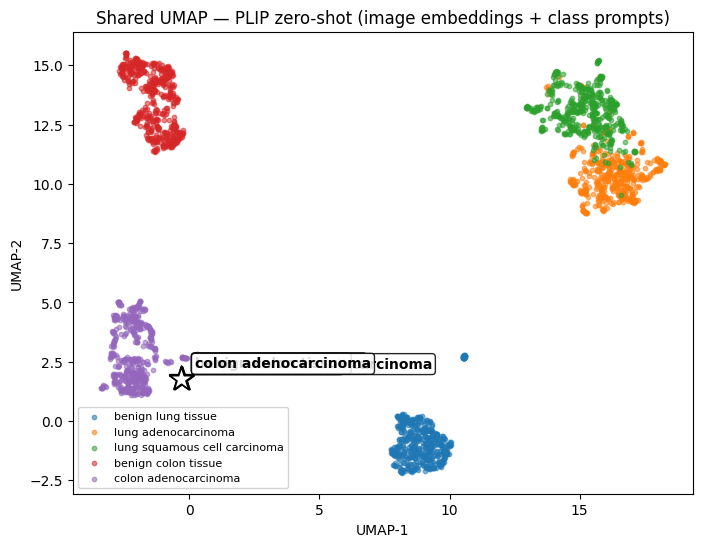
\includegraphics[width=\textwidth]{../results/plots/plip_zeroshot_umap.png}
        \par\vspace{2pt}\footnotesize (a) PLIP zero-shot.
    \end{minipage}\hfill
    \begin{minipage}[t]{0.48\textwidth}
        \centering
        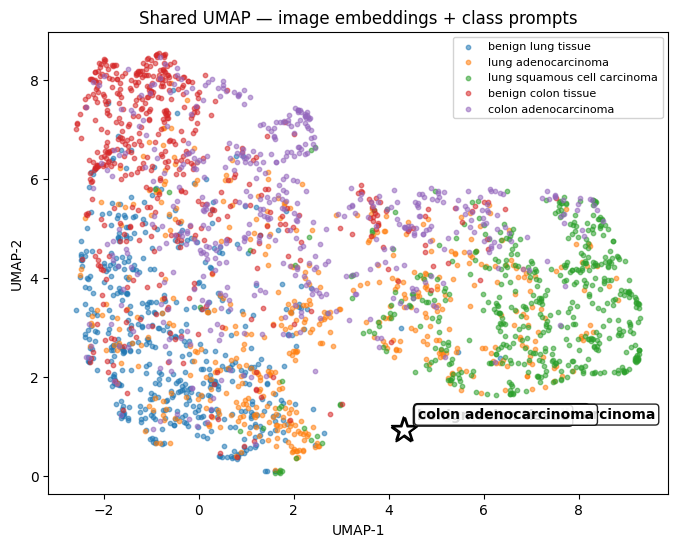
\includegraphics[width=\textwidth]{../results/plots/baseline_umap.png}
        \par\vspace{2pt}\footnotesize (b) Baseline (for comparison).
    \end{minipage}
    \caption{Training-source UMAP comparison. PLIP zero-shot (a) shows visibly tighter, more separated class clusters than the baseline (b) without any LC25000 supervision --- the gain is image-side.}
    \label{fig:plip-umap}
\end{figure}

\subsection{Generalization to external datasets}

\begin{table}[ht]
    \centering
    \small
    \begin{tabular}{|l|c|c|c|c|}
    \hline
    \textbf{Dataset (organ)} & \textbf{Macro-F1} & \textbf{Accuracy} & \textbf{Bal.\ acc.} & \textbf{Weighted F1} \\ \hline
    NCT-CRC-HE-7K (colon)            & 0.661 & 0.557 & 0.610 & 0.679 \\ \hline
    Chaoyang (colon)                 & \textbf{0.731} & 0.737 & 0.761 & 0.727 \\ \hline
    LungHist700 (lung, 20$\times$)   & 0.544 & 0.621 & 0.567 & 0.583 \\ \hline
    \end{tabular}
    \caption{PLIP zero-shot generalization across the three external datasets. No LC25000 supervision; class prediction by cosine similarity to PLIP-encoded prompts.}
    \label{tab:plip-zeroshot-ood}
\end{table}

\begin{itemize}
    \item \textbf{Chaoyang $>$ NCT.} PLIP zero-shot scores higher on Chaoyang ($0.731$) than on NCT-CRC ($0.661$), opposite of the pattern for every LC25000-trained variant (where NCT is the easier external dataset). Plausible reason: NCT-CRC is Macenko-normalised at release, pushing it away from the natural-staining distribution PLIP saw in OpenPath; Chaoyang's natural-stain images are stylistically closer to PLIP's pretraining corpus.
    \item \textbf{LungHist700 $= 0.544$.} The interesting cell. PLIP zero-shot has no LC25000 lung supervision yet outperforms the LC25000-trained ResNet50 variants ($0.305$) by $+0.239$ F1 on lung. Per-class recall: benign $0.16$ / AdC $0.69$ / SqC $0.84$ --- biased toward squamous like the ResNet50 variants, but not nearly as collapsed.
    \item Smallest training-source $\to$ external drop overall ($-0.04$ on NCT) --- the ``pretrained generalist'' pattern: never the best, never the worst, but consistent across distributions.
\end{itemize}

\subsection{What we learned}
\begin{itemize}
    \item Pathology pretraining produces a \emph{meaningfully better image representation} (visible directly in the UMAP) even without LC25000 supervision.
    \item PLIP's off-the-shelf prompt geometry is weak for our specific 5-class LC25000 vocabulary --- this decouples ``the image representation is useful'' from ``the off-the-shelf classifier works''.
    \item Section~\ref{sec:results-image-encoder} returns to this distinction by keeping PLIP's image representation but replacing its prompt geometry with a projection head trained on LC25000.
\end{itemize}


% ============================================================
\section{Foundational model vs plain classifier}
\label{sec:results-foundational-vs-plain}

\subsection{Configuration}
\begin{itemize}
    \item Same frozen ResNet50 image encoder as the baseline.
    \item Drops the CLIP paradigm entirely: no text encoder, no projection heads, no learnable temperature, no contrastive loss.
    \item Replaces it with a non-CLIP closed-set classifier: ResNet50 $\to$ global average pooling $\to$ BatchNorm $\to$ Dense(5) trained with sparse cross-entropy.
    \item Isolates what the CLIP paradigm itself contributes once the image encoder, data, and adaptation budget are held constant. Tests RQ2 (the foundational-model premise).
\end{itemize}

\subsection{Training source results}
\begin{itemize}
    \item Macro-F1 on LC25000: \textbf{0.6369} (vs baseline $0.6273$) \textit{(both numbers pre-bug-fix; post-fix both saturate at $\sim 0.99$, indistinguishable in-distribution)}.
    \item In-distribution the two architectures tie within noise. The choice between contrastive (CLIP) and direct supervised (plain classifier) is invisible when the image features are fixed and the training distribution is the evaluation distribution.
\end{itemize}

\subsection{Generalization to external datasets}
\begin{table}[ht]
    \centering
    \small
    \begin{tabular}{|l|c|c|c|c|}
    \hline
    \textbf{Variant} & \textbf{LC25000} & \textbf{NCT} & \textbf{Chaoyang} & \textbf{LungHist700} \\ \hline
    Baseline (CLIP InfoNCE)   & 0.996 & 0.866          & \textbf{0.786} & \textbf{0.305} \\ \hline
    Plain classifier (CE)     & 0.995 & \textbf{0.880} & 0.722          & 0.281 \\ \hline
    $\Delta$ (CLIP $-$ plain) & $-0.001$ & $-0.014$ & $+0.064$ & $+0.024$ \\ \hline
    \end{tabular}
    \caption{CLIP (baseline) vs plain classifier on the same frozen ResNet50 image encoder, macro-F1 across the training-source test split and three external datasets.}
    \label{tab:clip-vs-plain}
\end{table}

\begin{itemize}
    \item \textbf{Training source}: tied at $\sim 0.99$ (saturation null).
    \item \textbf{NCT-CRC (closest external dataset)}: plain CE marginally ahead by $+0.014$ F1.
    \item \textbf{Chaoyang (harder external)}: CLIP ahead by $+0.064$ F1 --- plain CE drops to last.
    \item \textbf{LungHist700 (hardest external)}: both variants collapse near 3-class chance; CLIP retains a marginal edge.
\end{itemize}

\noindent\textbf{Per-class signature on Chaoyang.} Plain CE shows benign precision $0.96$, benign recall $0.47$ (high precision, low recall --- the classifier is rarely predicting benign but is right when it does); adenocarcinoma precision $0.70$, recall $0.98$. The plain classifier is almost-degenerate ``predict adenocarcinoma'' under shift. The baseline CLIP variant is imperfect but balanced (benign $0.86$/$0.65$, adeno $0.76$/$0.92$), avoiding the collapse.

\subsection{What we learned}
\begin{itemize}
    \item CLIP and plain CE are \emph{interchangeable on easy distributions}; the choice of architecture is invisible when the model is evaluated on its training distribution.
    \item CLIP's edge appears \emph{under shift severity and grows with it}: $-0.014$ F1 on close-shift NCT (plain ahead), $+0.064$ on different-hospital Chaoyang (CLIP ahead), $+0.024$ on different-source LungHist700.
    \item \textbf{Mechanism}: same image encoder, same image features. The difference is the classifier geometry. The plain CE softmax learns class \emph{direction vectors} in feature space and is trained to maximise the logit margin; on shifted data those vectors don't move but the inputs sit in different regions, and the high-confidence softmax collapses into a single-class predictor. CLIP uses cosine similarity to class-prompt embeddings in an L2-normalized 256-d projection space, scaled by a learned temperature. Three effects make this geometry more robust:
    \begin{itemize}
        \item Cosine similarity is bounded in $[-1, 1]$ --- no unbounded margin for the model to over-extrapolate.
        \item The L2-normalized space concentrates features near the unit sphere; samples that drift in absolute feature space remain closer in \emph{angular} terms to the prompt anchors.
        \item The learned temperature $\tau$ acts as a soft regularizer on the cosine distribution: it tempers extreme confidence without removing the ranking signal.
    \end{itemize}
    \item This is a property of the CLIP \emph{paradigm}, not of any specific encoder. The same geometry was designed for the open-vocabulary regime (new class prompts at inference time) and incidentally protects against distribution shift on closed-set tasks. \textbf{This validates RQ2's foundational-model framing}: CLIP earns its complexity not at peak in-distribution accuracy, but in the open-vocabulary capabilities (retrieval, prompt-tuning at inference) and the robustness-under-shift behaviour shown here.
\end{itemize}


% ============================================================
\section{Text encoder pretraining}
\label{sec:results-text-encoder}

\subsection{Configuration}
\begin{itemize}
    \item Same arch / loss / prompts / split as the baseline; only the frozen text encoder changes.
    \item Three encoders: \texttt{bert-base-uncased} (the baseline's text encoder), BioBERT, PubMedBERT.
    \item Two prompt strategies: \textbf{name\_only} (just the class name, e.g.\ \texttt{``benign lung tissue''}) and \textbf{composed} (\texttt{``A histopathology image of \{class\}.''}, the baseline format).
    \item $3 \times 2 = 6$ cells. All three encoders are BERT-family, all produce 768-d hidden state, all tokenize through BERT-family WordPiece tokenizers.
    \item Tests RQ4 (does biomedical text pretraining help under short class-name prompts?).
\end{itemize}

\subsection{NCT-CRC grid (6 cells)}
\begin{table}[ht]
    \centering
    \small
    \begin{tabular}{|l|c|c|c|}
    \hline
    \textbf{Cell} & \textbf{LC25000} & \textbf{NCT-CRC} & \textbf{$\Delta$ vs baseline NCT} \\ \hline
    BERT + name\_only       & 0.999 & 0.821 & $-0.045$ \\ \hline
    BERT + composed         & 0.999 & 0.863 & $-0.003$ \\ \hline
    BioBERT + name\_only    & 0.998 & 0.840 & $-0.026$ \\ \hline
    BioBERT + composed      & 0.998 & 0.818 & $-0.048$ \\ \hline
    PubMedBERT + name\_only & 0.995 & 0.855 & $-0.011$ \\ \hline
    PubMedBERT + composed   & 0.996 & 0.808 & $-0.058$ \\ \hline
    \end{tabular}
    \caption{6-cell biomedical text encoder ablation, macro-F1 on NCT-CRC. \textbf{None of the 6 cells beats the baseline ($0.866$ on NCT).} LC25000 in-distribution saturates uniformly; all generalization numbers land in the $0.81$--$0.86$ band. The BERT + composed cell is essentially baseline (same architecture, same prompt template); the best \emph{biomedical} cell --- PubMedBERT + name\_only at $0.855$ --- still trails baseline by $-0.011$ F1.}
    \label{tab:text-encoder}
\end{table}

\begin{figure}[ht]
    \centering
    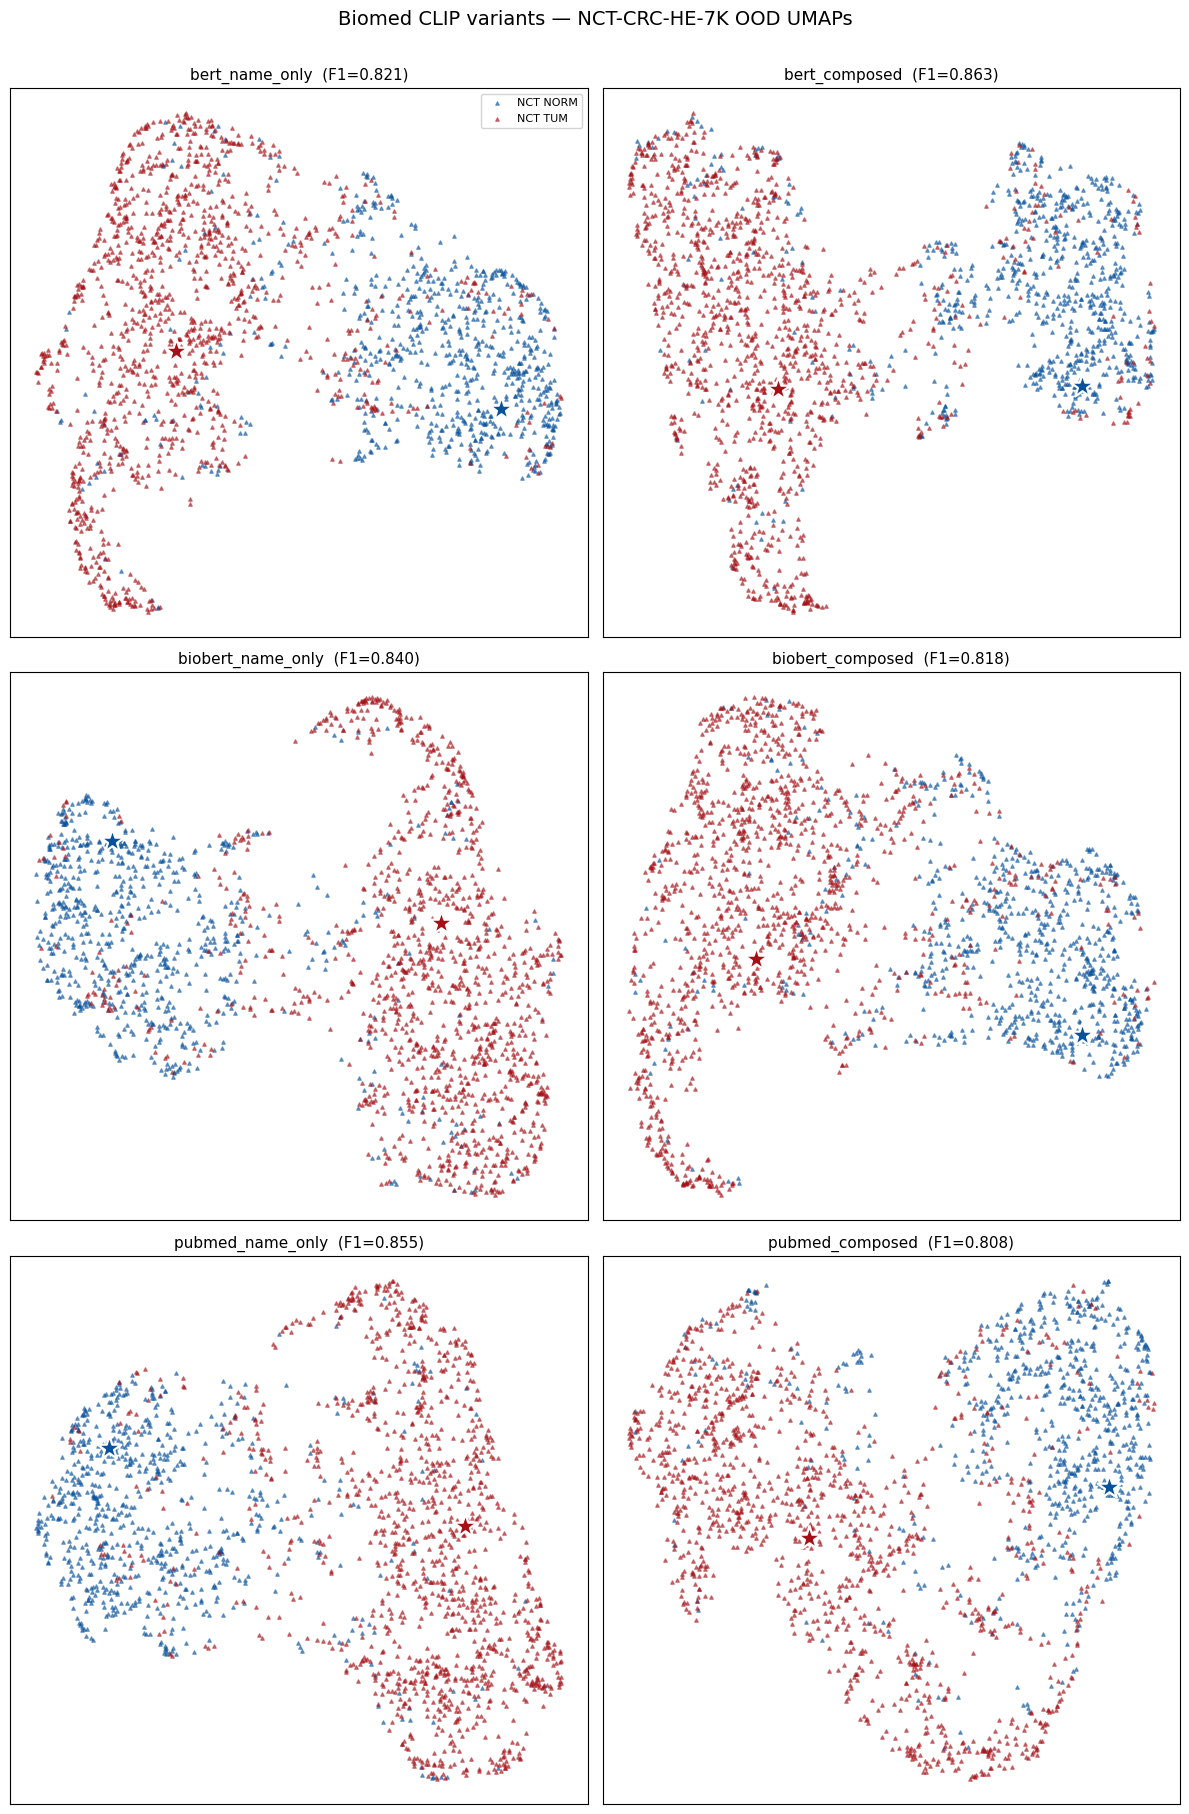
\includegraphics[width=0.95\textwidth]{../results/plots/exp_07_ood_eval/biomed_ood_umap_grid.png}
    \caption{6-cell UMAP grid (one panel per BERT/BioBERT/PubMedBERT $\times$ name\_only/composed cell), cross-distribution view on NCT-CRC. The clusters are qualitatively similar across cells, consistent with the lack of meaningful F1 separation in Table~\ref{tab:text-encoder}.}
    \label{fig:biomed-umap}
\end{figure}

\begin{itemize}
    \item LC25000 in-distribution: all cells saturate uniformly. The training-source axis does not discriminate these encoders.
    \item NCT generalization: all 6 cells land in the $0.81$--$0.86$ band. None beats the baseline.
\end{itemize}

\subsection{Generalization to Chaoyang and LungHist700}
\begin{itemize}
    \item The best biomedical cell on NCT --- PubMedBERT + name\_only --- was extended to Chaoyang and LungHist700 to test whether biomedical text encoders carry any advantage under heavier shift:
\end{itemize}

\begin{table}[ht]
    \centering
    \small
    \begin{tabular}{|l|c|c|c|}
    \hline
    \textbf{External dataset} & \textbf{Baseline F1} & \textbf{PubMedBERT+name\_only F1} & \textbf{Delta} \\ \hline
    NCT-CRC-HE-7K (close-shift colon)               & $0.866$ & $0.855$ & $-0.011$ \\ \hline
    Chaoyang (different-hospital colon)             & $0.786$ & $0.795$ & $+0.009$ \\ \hline
    LungHist700 (different-source lung, 20$\times$)  & $0.305$ & $0.279$ & $-0.026$ \\ \hline
    \end{tabular}
    \caption{Best biomedical text-encoder cell (PubMedBERT + name\_only) vs baseline on the three external evaluation datasets. The biomedical text encoder ties baseline on Chaoyang (within noise) and regresses on both NCT and LungHist700. No measurable transfer benefit on any of the three datasets.}
    \label{tab:text-encoder-3way}
\end{table}

\begin{itemize}
    \item \textbf{No transfer.} The best biomedical cell ties baseline on Chaoyang ($+0.009$, within noise) and \emph{regresses} on LungHist700 ($-0.026$). Combined with the NCT result ($-0.011$), no biomedical-text-encoder configuration tested produces a measurable gain on any external dataset.
    \item \textbf{LungHist700 collapse signature.} Both baseline and PubMedBERT+name\_only collapse on lung, just to different classes. Baseline predicts ``lung squamous cell carcinoma'' on most inputs in the degenerate regime; PubMedBERT+name\_only also collapses to lung\_scc but harder ($\sim 92$\% of predictions). In both cases the per-class recall on the other two lung classes is near-zero --- a single-class predictor regime where the text encoder choice only affects how \emph{sharply} the collapse manifests.
\end{itemize}

\subsection{What we learned}
\begin{itemize}
    \item Biomedical text pretraining does \emph{not} help on this task at frozen-backbone scale with short class-name prompts. Confirmed across three external datasets: PubMedBERT + name\_only (the best biomedical cell on NCT) ties baseline on Chaoyang and regresses on both NCT and LungHist700.
    \item \textbf{Mechanism --- why doesn't ``a more domain-aware text encoder'' improve results?} Three converging reasons:
    \begin{itemize}
        \item \emph{The projection head absorbs encoder-specific differences.} BERT, BioBERT, and PubMedBERT all start from different 768-d embedding spaces, but they all get pulled through the same projection head trained on LC25000. The head learns to map any reasonable starting embedding to useful class anchors. With only 5 LC25000 classes to separate, this is an easy adaptation regardless of where the starting embeddings sit.
        \item \emph{Short class-name prompts don't expose biomedical-vocabulary richness.} Biomedical pretraining adds value most when domain vocabulary actually appears --- clinical notes, paper abstracts, multi-sentence text. Strings like \texttt{``colon adenocarcinoma''} tokenize into 2--3 wordpieces that any BERT-family encoder handles competently. There is no rare-medical-term upside for biomedical pretraining to surface.
        \item \emph{CLIP's shift robustness is geometric, not domain-knowledge driven.} As argued in Section~\ref{sec:results-foundational-vs-plain}, CLIP's edge under shift comes from the cosine + L2-norm + temperature classifier geometry, which is independent of the text encoder. Swapping in a more medically-aware text encoder doesn't change the classifier geometry; it changes the starting position of the prompt anchors, which the projection head then re-maps anyway.
    \end{itemize}
    \item \textbf{Small but interesting secondary observation}: vanilla BERT prefers the longer \textbf{composed} prompt format; biomedical encoders prefer \textbf{bare class names}. Plausible mechanism: biomedical pretraining made strings like \texttt{``colon adenocarcinoma''} carry strong signal on their own, while adding generic boilerplate (\texttt{``A histopathology image of \ldots''}) dilutes the prompt embedding for biomedical encoders. Not enough to flip any cell to winning --- but a useful methodological note for short-prompt design.
\end{itemize}


% ============================================================
\section{Image encoder pretraining}
\label{sec:results-image-encoder}

\subsection{Configuration}
\begin{itemize}
    \item Same arch / loss / prompts / split / text encoder (frozen BERT base) as the baseline. The only axis that changes is the image encoder's pretraining.
    \item Three image encoders compared, all frozen, trainable parameters limited to the projection head + temperature:
    \begin{itemize}
        \item \textbf{ResNet50 (general-purpose, ImageNet pretraining)} --- the baseline.
        \item \textbf{Visual Transformer (ViT-B/32) with PLIP's OpenPath pretraining} --- a ViT pretrained on $\sim$208k histopathology image--text pairs scraped from Twitter.
        \item \textbf{Visual Transformer (ViT-B/14) with DINOv2 self-supervised pretraining} --- a ViT pretrained on $\sim$142M curated general natural images via self-distillation, no labels, no histopathology data.
    \end{itemize}
    \item \textbf{Role of DINOv2 in the comparison}: a control. PLIP differs from the baseline on multiple axes simultaneously (architecture: ViT vs CNN; objective: contrastive vs supervised; pretraining domain: histopathology vs natural images). DINOv2 isolates the ``ViT + self-supervised on general data'' axis from the ``histopathology pretraining specifically'' axis. If DINOv2 also breaks the baseline's lung collapse, the win is partly architectural; if it does not, the win is specifically about histopathology pretraining.
    \item \textbf{Caveat}: the two ViTs differ in patch size (PLIP B/32, DINOv2 B/14). At 224$\times$224 input this gives different feature granularity (49 vs 256 patch tokens). We discuss this as a confound in Methodology and address it as a limitation in Chapter~5.
\end{itemize}

\subsection{Training source results}
\begin{itemize}
    \item PLIP image encoder + LC25000 supervision: LC25000 macro-F1 $= 0.996$. Same saturation null as every other trained variant.
    \item DINOv2 image encoder + LC25000 supervision: LC25000 macro-F1 $= 0.989$. The saturation null holds even though DINOv2 has never seen labelled histology --- its pretraining is self-supervised on general natural images, with no class labels. Confirms that the in-distribution null is backbone-independent: the bottleneck on the meaningful axis is not what the image encoder ``knows about histology'' in the supervised sense; it is what kind of variation the encoder learned to be sensitive to.
\end{itemize}

\subsection{Generalization to external datasets}
\begin{table}[ht]
    \centering
    \small
    \begin{tabular}{|l|c|c|c|c|}
    \hline
    \textbf{Image encoder} & \textbf{LC25000} & \textbf{NCT} & \textbf{Chaoyang} & \textbf{LungHist700} \\ \hline
    ResNet50 (ImageNet)                              & 0.996 & 0.866 & 0.786 & 0.305 \\ \hline
    ViT-B/14 (DINOv2 / self-supervised)              & 0.989 & 0.855 & 0.776 & 0.457 \\ \hline
    \textbf{ViT-B/32 (PLIP / OpenPath)}              & \textbf{0.996} & \textbf{0.933} & \textbf{0.813} & \textbf{0.640} \\ \hline
    \end{tabular}
    \caption{Image encoder pretraining swap, macro-F1 across the training-source split and three external datasets. Everything except the image encoder is identical across rows.}
    \label{tab:image-encoder}
\end{table}

\begin{itemize}
    \item \textbf{NCT-CRC (close-shift colon)}: PLIP wins by $+0.067$ F1 over the ResNet50 baseline. DINOv2 lands at $-0.011$ vs baseline --- general-domain self-supervision does \emph{not} help on the easiest external dataset. The colon ceiling around $0.88$ that none of the other interventions could clear is broken specifically by changing the image encoder's pretraining \emph{domain}, not by architecture or self-supervision alone.
    \item \textbf{Chaoyang (different-hospital colon)}: PLIP wins by $+0.027$ F1; DINOv2 lands at $-0.010$ vs baseline. Same colon-side pattern as NCT: only histopathology pretraining helps; general SSL is interchangeable with ImageNet supervision.
    \item \textbf{LungHist700 (different-source lung)}: this is where the control pays off. PLIP wins by $+0.335$ F1 over baseline; DINOv2 wins by $+0.152$ F1. \emph{Roughly half of PLIP's lung advantage comes from architecture + self-supervised pretraining on general images; the other half comes from histopathology pretraining specifically.} DINOv2 partially rescues the lung collapse (per-class recall $0.46/0.52/0.40$, balanced) but does not match PLIP's full functional classifier ($0.51/0.49/0.91$).
\end{itemize}

\noindent\textbf{Per-class signature on LungHist700.} Both ResNet50 variants converge to the same degenerate predictor on lung tissue: baseline recall $0.19/0.07/0.89$ for normal/AdC/SqC, plain CE $0.15/0.05/0.91$ --- both predict ``squamous'' on $\sim 90$\% of inputs regardless of true class. \textbf{DINOv2-encoded variant: $0.46/0.52/0.40$} --- balanced across all 3 classes, no degenerate collapse, but lower peak per-class scores than PLIP. \textbf{PLIP-encoded variant: $0.51/0.49/0.91$} --- balanced \emph{and} retains the high squamous recall, the only variant that does both.

\begin{figure}[ht]
    \centering
    \begin{minipage}[t]{0.48\textwidth}
        \centering
        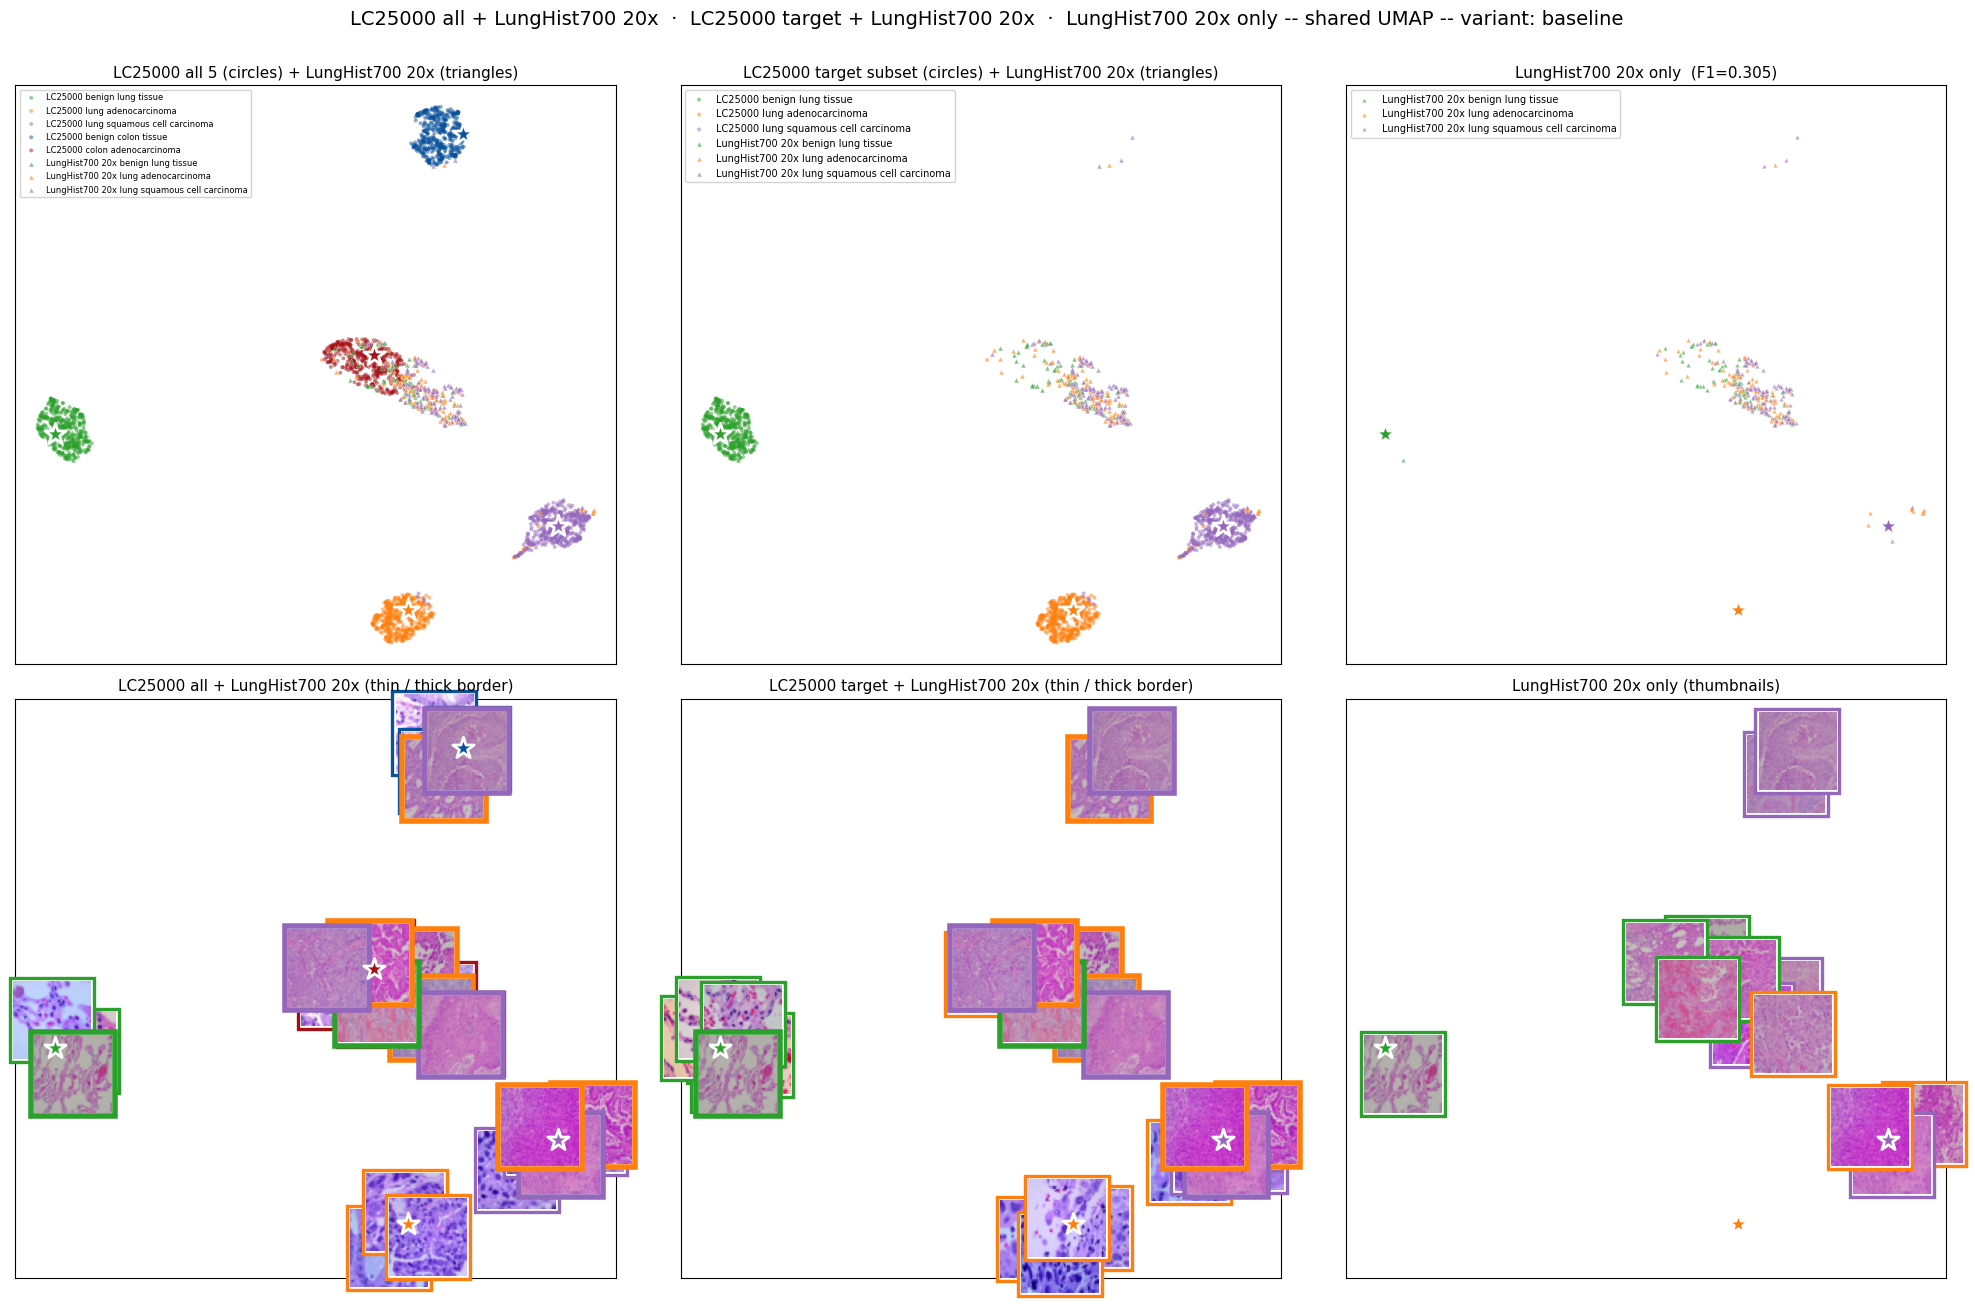
\includegraphics[width=\textwidth]{../results/plots/exp_07_ood_eval/baseline_lunghist700_20x_ood_umap_grid.png}
        \par\vspace{2pt}\footnotesize (a) ResNet50 baseline: a single tight blob, no internal class structure.
    \end{minipage}\hfill
    \begin{minipage}[t]{0.48\textwidth}
        \centering
        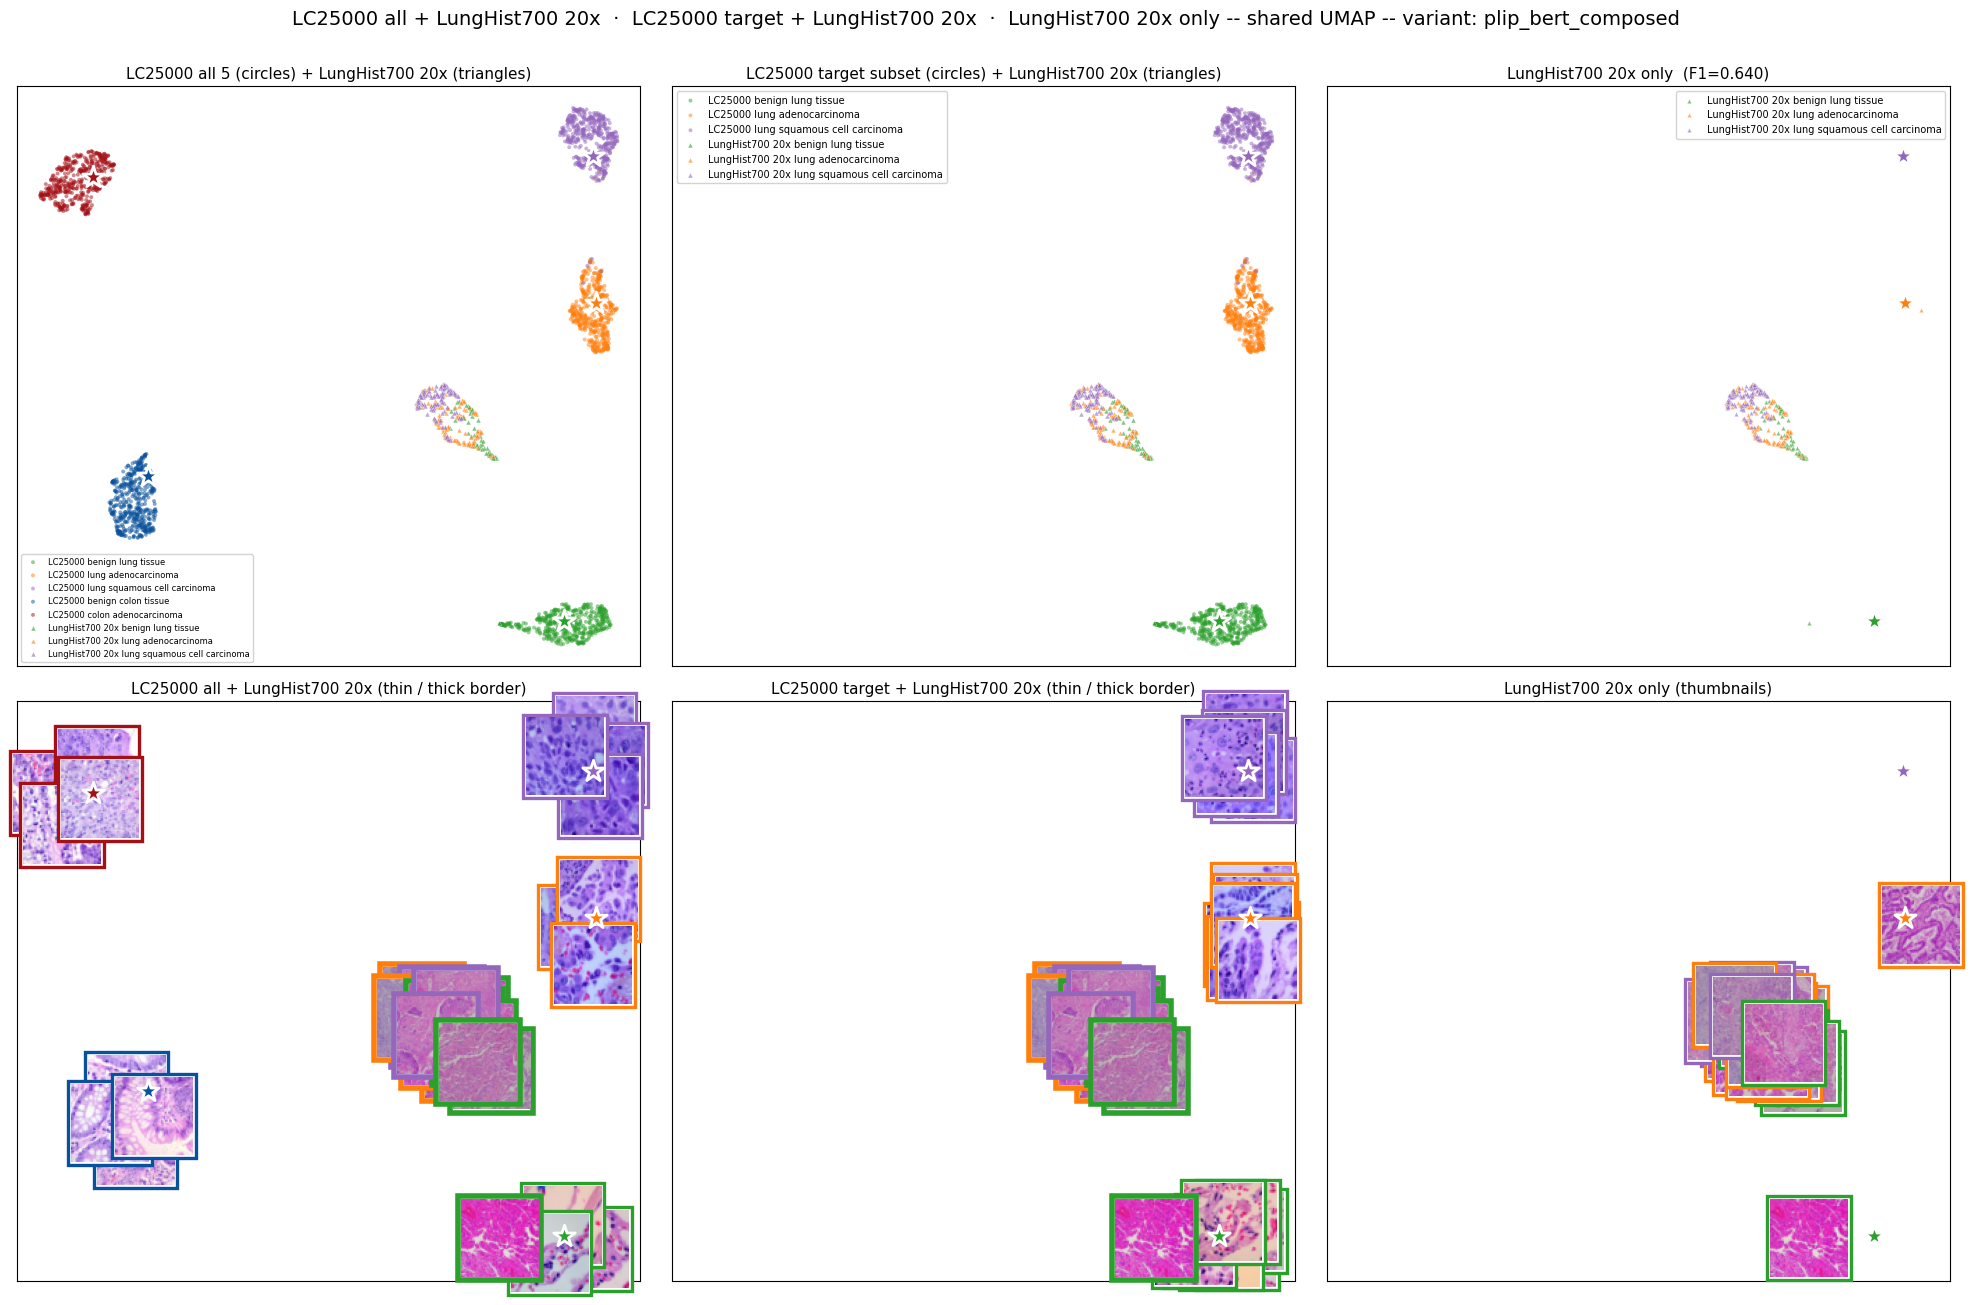
\includegraphics[width=\textwidth]{../results/plots/exp_07_ood_eval/plip_bert_composed_lunghist700_20x_ood_umap_grid.png}
        \par\vspace{2pt}\footnotesize (b) ViT-B/32 with PLIP pretraining: three visibly separated sub-clusters by class.
    \end{minipage}
    \caption{LungHist700 cross-distribution UMAP comparison --- the visual headline of this chapter. The ResNet50 baseline (a) places all 359 LungHist700 samples into a single tight cluster with no internal class structure; the PLIP-pretrained ViT (b) produces three visibly distinct sub-clusters by class, sitting adjacent to (but not co-located with) the matching LC25000 lung clusters.}
    \label{fig:image-encoder-umap-lung}
\end{figure}

\subsection{What we learned}
\begin{itemize}
    \item The \textbf{image encoder's pretraining is the dominant lever in this study}, but the DINOv2 control reveals that ``pretraining'' decomposes into two contributing components.
    \item Effect-size summary: PLIP gains over baseline by $+0.067$ F1 on close-shift colon, $+0.027$ on different-hospital colon, \textbf{$+0.335$ on different-source lung}. DINOv2 gains over baseline by $-0.011$ / $-0.010$ / $+0.152$ on the same three datasets.
    \item \textbf{On colon (NCT, Chaoyang)}: only histopathology pretraining moves the needle. General-domain self-supervised pretraining (DINOv2) lands within noise of ResNet50 supervised pretraining on natural images. The colon advantage is specifically about \emph{what} the encoder was pretrained on, not \emph{how}.
    \item \textbf{On lung (LungHist700)}: the DINOv2 and PLIP-zero-shot controls together yield a clean three-step decomposition of PLIP-backbone's $+0.335$ F1 gap. Baseline at $0.305$ $\to$ DINOv2 at $0.457$ ($+0.152$, ``ViT $+$ general-domain SSL'' contribution) $\to$ PLIP zero-shot at $0.544$ ($+0.087$, ``histopathology pretraining without LC25000 supervision'' contribution) $\to$ PLIP-backbone at $0.640$ ($+0.096$, ``LC25000 supervision on top of histopathology pretraining'' contribution). Three roughly comparable steps of $\sim 0.1$ F1 each, sequentially adding architecture/SSL, then domain, then task supervision.
    \item Why colon and lung behave differently, on the ResNet50 baseline: ImageNet supervision contains no histology. LC25000 supervision rescues ResNet50 features that happen to correlate with colon class labels in the LC25000 training distribution. That correlation transfers partially to NCT/Chaoyang (both colon, stylistically close). It does not transfer to lung tissue at all --- the lung-side ``success'' in-distribution is memorisation on the LC25000 lung subset, not learned lung tissue features.
    \item Why DINOv2 helps on lung but not colon: DINOv2's self-supervised pretraining on $\sim 142$M diverse natural images produces image features that are sensitive to a much broader range of local-texture variation than supervised ImageNet pretraining. That broader feature space provides \emph{enough} signal for LC25000 supervision + the projection head to construct a usable lung classifier, even though the encoder has never seen histology. On colon, where ResNet50 features were already enough for partial transfer, DINOv2's broader features do not help further --- the bottleneck on colon is the pretraining domain, not the architecture's feature breadth.
    \item Patch-size confound check: DINOv2 has more spatial detail than PLIP ($256$ vs $49$ patch tokens at the same 224$\times$224 input), but still loses on colon. The patch-size difference is therefore not the dominant factor here --- pretraining is.
\end{itemize}


% ============================================================
\section{Discussion}
\label{sec:results-discussion}

\subsection{Synthesis across experiments}
\begin{itemize}
    \item This chapter evaluated six interventions on a frozen general-purpose CLIP pipeline (ResNet50 + BERT). Five of the six (stain normalization, biomedical text encoders, plain-classifier substitution, the prompt-format variations within the text-encoder ablation) produce changes within $\sim 0.03$ F1 of the baseline on close-shift external evaluation (NCT) and at most $\sim 0.03$ F1 of improvement on the harder external datasets. Stain Macenko is the only input-side lever that moves the needle positively under shift ($+0.030$ on Chaoyang, $+0.020$ on LungHist700), but its magnitude is dominated by the image-encoder lever on the same datasets. The best biomedical text-encoder cell (PubMedBERT + name\_only) confirms the null result across all 3 external datasets --- ties baseline on Chaoyang, regresses on NCT and LungHist700.
    \item The sixth intervention --- replacing the image encoder's pretraining (Section~\ref{sec:results-image-encoder}) --- moves the headline metric by $+0.067$ on close-shift colon (NCT), $+0.027$ on different-hospital colon (Chaoyang), and \textbf{$+0.335$ on different-source lung (LungHist700)}, taking the lung result from a degenerate single-class predictor at $0.305$ to a functional 3-class classifier at $0.640$.
    \item The DINOv2 and PLIP-zero-shot controls together decompose that gain on lung into a clean ladder: $0.305$ (baseline) $\to$ $0.457$ (DINOv2: ViT $+$ SSL contribution, $+0.152$) $\to$ $0.544$ (PLIP zero-shot: histopath pretraining contribution, $+0.087$) $\to$ $0.640$ (PLIP-backbone: LC25000 supervision on top, $+0.096$). Three roughly equal steps of $\sim 0.1$ F1. On colon, the decomposition collapses --- DINOv2 ties baseline and PLIP zero-shot actually falls below baseline on Chaoyang ($0.731$ vs $0.786$) because LC25000 supervision was already enough.
    \item \textbf{The image encoder's pretraining is the dominant lever}, by roughly $5\times$ over the next-largest single lever on colon external evaluation. On lung, no head/loss/text-side intervention rescues a non-functional predictor at all; only changing the encoder does.
    \item The contemporary methods literature's emphasis on novel loss functions, text-side innovations, and stain harmonisation is not supported by this study at the frozen-backbone scale we evaluated.
\end{itemize}

\subsection{Secondary observations}
\begin{itemize}
    \item \textbf{Cross-organ regime change.} ResNet50 variants partially work on colon external data ($0.78$--$0.88$) but \emph{categorically fail} on lung ($\sim 0.30$, near 3-class chance). Mechanism: LC25000 supervision can rescue ResNet50 features that happen to correlate with colon class labels in LC25000, but cannot produce useful lung-tissue features within a frozen ImageNet ResNet50; the in-distribution lung ``success'' is memorisation. Per-organ external evaluation is therefore essential; aggregating across datasets hides the regime change.
    \item \textbf{Classification quality $\neq$ representation alignment.} Baseline CLIP achieves cross-dataset \emph{cluster alignment} but lower classification F1; PLIP achieves the highest F1 but leaves external samples in their own region of feature space. The contrastive objective optimises same-class-pair alignment; the cosine-classifier rule only needs alignment to the class-prompt direction. These are different geometric properties --- the right tradeoff depends on whether the downstream task is classification or representation-driven (retrieval, clustering, transfer).
    \item \textbf{Plain-classifier flip under shift.} Plain CE ties CLIP in-distribution and marginally wins NCT, but loses Chaoyang ($+0.064$ for CLIP) and LungHist700 ($+0.024$). High-confidence softmax classifiers degenerate into single-class predictors as shift severity grows (visible in the Chaoyang per-class signature); CLIP's cosine geometry doesn't. This supports the foundational-model framing of RQ2: CLIP earns its complexity in shift robustness, not in-distribution accuracy.
\end{itemize}

\subsection{Headline summary}
\begin{table}[ht]
    \centering
    \small
    \begin{tabular}{|l|c|c|c|c|}
    \hline
    \textbf{Variant} & \textbf{LC25000} & \textbf{NCT} & \textbf{Chaoyang} & \textbf{LungHist700} \\ \hline
    \textbf{ViT-B/32 (PLIP)}                  & \textbf{0.996} & \textbf{0.933} & \textbf{0.813} & \textbf{0.640} \\ \hline
    ViT-B/14 (DINOv2)                          & 0.989 & 0.855 & 0.776 & 0.457 \\ \hline
    Baseline (ResNet50 + BERT)                & 0.996 & 0.866 & 0.786 & 0.305 \\ \hline
    Plain CE classifier                        & 0.995 & 0.880 & 0.722 & 0.281 \\ \hline
    Stain Macenko (NCT-NORM reference)        & 0.986 & 0.844 & 0.816 & 0.325 \\ \hline
    Best biomedical text-encoder cell (PubMedBERT + name\_only) & 0.995 & 0.855 & 0.795 & 0.279 \\ \hline
    PLIP zero-shot (no LC25000 supervision)   & 0.700 & 0.661 & 0.731 & 0.544 \\ \hline
    \end{tabular}
    \caption{Headline summary across the chapter. PLIP-pretrained ViT wins every external evaluation; the lung-side advantage ($+0.335$ F1 over baseline) is an order of magnitude larger than the colon-side advantages. DINOv2 (the same-architecture, general-domain self-supervised control) lands between baseline and PLIP on lung but ties baseline on colon, decomposing PLIP's lung advantage into roughly equal architecture/SSL and histopathology-pretraining contributions. Stain Macenko (NCT-NORM) helps on the two datasets that arrive in their native stain palette (Chaoyang $+0.030$, LungHist700 $+0.020$) and regresses on NCT ($-0.022$), which arrives already Macenko-normalised at release. The best biomedical text-encoder cell (PubMedBERT + name\_only) ties baseline on Chaoyang and regresses on both NCT and LungHist700 --- no measurable transfer benefit on any of the three datasets. Limitations and future work are discussed in Chapter~5.}
    \label{tab:summary-headline}
\end{table}
